% Options for packages loaded elsewhere
\PassOptionsToPackage{unicode}{hyperref}
\PassOptionsToPackage{hyphens}{url}
%
\documentclass[
]{article}
\usepackage{amsmath,amssymb}
\usepackage{lmodern}
\usepackage{iftex}
\ifPDFTeX
  \usepackage[T1]{fontenc}
  \usepackage[utf8]{inputenc}
  \usepackage{textcomp} % provide euro and other symbols
\else % if luatex or xetex
  \usepackage{unicode-math}
  \defaultfontfeatures{Scale=MatchLowercase}
  \defaultfontfeatures[\rmfamily]{Ligatures=TeX,Scale=1}
  \setmainfont{Noto Serif CJK SC}
  \setsansfont{DejaVu Sans}
  \setmonofont{DejaVu Sans Mono}
  \IfFileExists{xeCJK.sty}{%
    \usepackage{xeCJK}
    \setCJKmainfont{Noto Serif CJK SC}
    \setCJKsansfont{Noto Sans CJK SC}
  }{}
  \IfFileExists{ucharclasses.sty}{%
    \usepackage{ucharclasses}
    \newfontfamily\CJKfont{Noto Serif CJK SC}[BoldFont={Noto Serif CJK SC Bold}]
    \setTransitionsForCJK{\CJKfont}{\rmfamily}
  }{}
\fi
% Use upquote if available, for straight quotes in verbatim environments
\IfFileExists{upquote.sty}{\usepackage{upquote}}{}
\IfFileExists{microtype.sty}{% use microtype if available
  \usepackage[]{microtype}
  \UseMicrotypeSet[protrusion]{basicmath} % disable protrusion for tt fonts
}{}
\makeatletter
\@ifundefined{KOMAClassName}{% if non-KOMA class
  \IfFileExists{parskip.sty}{%
    \usepackage{parskip}
  }{% else
    \setlength{\parindent}{0pt}
    \setlength{\parskip}{6pt plus 2pt minus 1pt}}
}{% if KOMA class
  \KOMAoptions{parskip=half}}
\makeatother
\usepackage{xcolor}
\IfFileExists{xurl.sty}{\usepackage{xurl}}{} % add URL line breaks if available
\IfFileExists{bookmark.sty}{\usepackage{bookmark}}{\usepackage{hyperref}}
\hypersetup{
  hidelinks,
  pdfcreator={LaTeX via pandoc}}
\urlstyle{same} % disable monospaced font for URLs
\usepackage{graphicx}
\makeatletter
\def\maxwidth{\ifdim\Gin@nat@width>\linewidth\linewidth\else\Gin@nat@width\fi}
\def\maxheight{\ifdim\Gin@nat@height>\textheight\textheight\else\Gin@nat@height\fi}
\makeatother
% Scale images if necessary, so that they will not overflow the page
% margins by default, and it is still possible to overwrite the defaults
% using explicit options in \includegraphics[width, height, ...]{}
\setkeys{Gin}{width=\maxwidth,height=\maxheight,keepaspectratio}
% Set default figure placement to htbp
\makeatletter
\def\fps@figure{htbp}
\makeatother
\usepackage[normalem]{ulem}
% Avoid problems with \sout in headers with hyperref
\pdfstringdefDisableCommands{\renewcommand{\sout}{}}
\setlength{\emergencystretch}{3em} % prevent overfull lines
\providecommand{\tightlist}{%
  \setlength{\itemsep}{0pt}\setlength{\parskip}{0pt}}
\setcounter{secnumdepth}{-\maxdimen} % remove section numbering
\ifLuaTeX
  \usepackage{selnolig}  % disable illegal ligatures
\fi

\author{}
\date{}

\begin{document}

\textbf{\sout{Droplet-engineered appendix-derived gut organoids enable controlled growth, differentiation and fusion}}

\textbf{AI segmentation reveals droplet-engineered appendix-derived gut organoids enable controlled growth, differentiation, and fusion}

\textbf{Agentic analysis of droplet-engineered appendix-derived gut organoid growth, differentiation, and fusion using AAPS}

\emph{Zhengyu Wu\textsuperscript{1, 3}, Rongzhou Chen \textsuperscript{2,3}, Wanlong Wang\textsuperscript{1}, Chuqian Ruan\textsuperscript{1}, Haotian Sun\textsuperscript{1}, Edmund Y. Lam\textsuperscript{2}, Shaohua Ma\textsuperscript{1,4}}

\begin{enumerate}
\def\labelenumi{\arabic{enumi}.}
\item
  Institute of Biopharmaceutical and Health Engineering (iBHE), Tsinghua Shenzhen International Graduate School (SIGS), Tsinghua University, Shenzhen 518055, China
\item
  Department of Electrical and Computer Engineering, University of Hong Kong, Pokfulam, Hong Kong SAR, China
\item
  These authors contributed equally
\item
  Corresponding Email: ma.shaohua@sz.tsinghua.edu.cn
\end{enumerate}

\textbf{Abstract}

Human intestinal organoid culture is strongly influenced by physical and biochemical parameters that govern epithelial growth, differentiation, and fusion. However, deciphering these regulatory cues remains challenging without quantitative assessment of culture conditions and phenotypic outcomes. Here, we establish a droplet-engineered organoid (DEO) platform using human appendix-derived gut organoids and systematically evaluate the effects of seeding density, alginate incorporation, and ROCK inhibition with Y-27632. We further use this dataset as a biomedical application of AAPS (Autonomous Agentic Pipeline Script), a prompt-native workflow harness that allows domain experts to express experimental design as top-down pipeline blocks with declared inputs, outputs, validation gates, artifacts, and human review. The AAPS Organoid Agent connected imaging metadata, image quality control, method routing, segmentation, metric design, and figure generation into auditable executable analysis outputs. Appendix-derived organoids were robustly established and used to generate DEOs. Our results show that seeding density regulates growth kinetics and fusion behavior, with middle to high density providing a more balanced growth pattern. Alginate-incorporated DEOs maintain cystic morphology longer and exhibit delayed epithelial wall thickening and reduced darkening compared to Matrigel controls, corroborated by RNA sequencing showing delayed differentiation. Y-27632 enhances DEO fusion in a dose-dependent manner while preserving cystic morphology. Collectively, our findings provide a practical framework for DEO optimization. More broadly, this study illustrates how a harnessed agentic workflow can convert heterogeneous organoid images into reproducible quantitative readouts by constraining agent decisions to small tasks, persistent artifacts, and expert-reviewed checkpoints.

\textbf{Keywords}

Droplet-engineered organoids; alginate; Y-27632; epithelial differentiation; fusion

\textbf{Introduction}

Human intestinal organoids are widely used as experimental models for epithelial biology, disease modeling, and regenerative studies because they recapitulate key structural and functional features of the intestinal epithelium {[}1-6{]}. However, conventional dome-based organoid cultures still face several limitations including substantial variability in size, morphology, and batch-to-batch consistency, making quantitative and standardized comparisons difficult across different experiment conditions {[}7, 8{]}. Such limitations are particularly relevant when organoids are intended for downstream applications that require structural reproducibility and precise control of epithelial state.

Droplet-engineered organoid (DEO) culture offers a promising strategy to improve organoid standardization. By incorporating organoid cells within microdroplets, DEOs can reduce matrix usage, increase throughput, and exert space regulations that may influence organoid growth, cell-cell interactions, differentiation and fusion {[}9-11{]}. Matrix composition is also likely to be an important determinant of these processes. Although Matrigel is widely used for epithelial growth, but its degradability and softness may allow organoids to expand in a less constrained manner {[}12{]}. In such systems, culture parameters are expected to play an important role in determining epithelial behavior, yet their effects have not been systematically evaluated.

The development of a useful DEO platform requires not only efficient organoid formation, but also controlled regulation of epithelial growth, lineage differentiation, and fusion-related tissue remodeling {[}13-16{]}. These features are biologically and technically important. Growth influences the efficiency and reproducibility of organoid expansion, differentiation reflects epithelial maturity, and fusion is particularly relevant in spatially restricted droplet systems, where close organoid-organoid contact may favor the formation of larger integrated epithelial structures {[}14{]}. A clearer understanding of how culture conditions govern these phenotypes is therefore essential for establishing a stable and tunable DEO platform.

Quantitative analysis is essential for evaluating DEO phenotypes, particularly in large brightfield imaging datasets. However, organoid brightfield images are often highly heterogeneous in size, morphology, density, magnification, background quality, and fusion state, making robust segmentation and standardized quantification challenging. A single fixed algorithm is therefore unlikely to remain optimal across all images and experimental branches. Conversely, an unconstrained AI agent is difficult to audit because method choices, intermediate assumptions, and failure recovery may remain implicit. This creates a need for a workflow layer that allows domain experts to describe the experiment in the language of biological design while still producing executable, inspectable, and reproducible analysis artifacts.

To address this problem, we implemented an AAPS Organoid Agent based on AAPS (Autonomous Agentic Pipeline Script). AAPS is a prompt-native and project-oriented workflow language and Studio that places AI agents inside a structured harness. In this model, a domain expert can design a pipeline from the top down, beginning with the experimental goal and metadata structure, then refining it into reusable blocks for imaging capture, quality control, image-prior extraction, method routing, segmentation, metric calculation, visualization, and reporting. Each block declares its inputs, outputs, artifacts, tools, validation rules, and review checkpoints. The AAPS Studio supports prompt-based construction and testing of reusable skills and blocks, while the compiler/runtime layer converts structured pipeline intent into project-local executable actions, setup or repair prompts, run manifests, logs, masks, overlays, metric tables, and reports.

This design also provides a practical answer to the consistency problem in agentic scientific analysis. We do not assume that a large language model alone guarantees reproducible behavior. Instead, AAPS reduces the scope of agentic decisions by decomposing the workflow into small, auditable tasks. The agent may help inspect an image, choose between Cellpose, thresholding, multiscale segmentation, or image-generation-assisted refinement, or draft a missing script; however, the output of each step is materialized as an artifact that can be checked. In the present study, segmentation masks, overlays, per-image metric JSON files, summary CSV files, and final plots were retained, and difficult cases were routed to human-in-the-loop review before inclusion in the final database. Thus, the consistency of the analysis arises from divide-and-conquer task design, artifact-level verification, provenance tracking, deterministic scripts where possible, and expert review where biological image ambiguity remains. Stronger formal benchmarking and automated consistency scoring remain important future directions.

In this study, we combined droplet-engineered human appendix-derived gut organoid culture with the AAPS Organoid Agent to systematically investigate how seeding density, alginate incorporation, and ROCK inhibition by Y-27632 regulate organoid growth, differentiation, and fusion. This DEO analysis provides a stringent application case for AAPS because the images span variable organoid size, density, morphology, fusion state, and brightfield quality, and because the biological conclusions depend on consistent extraction of growth-, differentiation-, and fusion-related features. We further performed bulk RNA sequencing to characterize transcriptomic changes associated with alginate-containing DEOs. Together, this work establishes a biologically informed and quantitatively analyzable DEO platform, while illustrating how a prompt-native agentic workflow harness can connect experimental design, image analysis, metric selection, and interpretable biological conclusions.

\textbf{Results}

\textbf{Establishment of appendix-derived organoids and DEO platform}

Appendix-derived gut organoids were successfully established from human tissues using nonengineered manual pipetting method (Figure 1A). These organoids served as the source material for DEO generation. To establish DEOs, crypts derived from nonengineered organoids (NEO) were embedded within Matrigel (Figure 1B). The continuous flow provided by uniform 0.56 mm inner diameter PTFE tubing supported stable droplet production, and droplets remained in same distance after formation at the T-junction. This method produced confined DEOs usually consisted of a single microdroplet with approximately 500 µm diameter and a volume of \textasciitilde0.1 µL. However, conventional organoid culture used the manual pipetting dome method, this may require use of a 50 µL Matrigel dome per well for the establishment of appendix-derived organoids. Thus, the droplet-engineering strategy can increase experimental throughput by more than two orders of magnitude while substantially reducing variability associated with manual handling. Also, the distinct geometric constraints of the DEO system are very likely to affect biological behavior {[}17, 18{]}. In DEOs, these cells are confined within a limited distance from the droplet center, promoting closer cell-cell distributions compared to conventional methods (Figure S1).

To support subsequent quantitative analysis, we first established a structured dataset-management workflow for DEO brightfield imaging (Figure 1C). Raw brightfield images were collected and subjected to image quality control and filtering before inclusion in the final analysis set. This step was designed to reduce the influence of low-quality or non-informative images and to improve the consistency of downstream analysis. The curated dataset was then organized into three experimental branches corresponding to the density, alginate, and Y-27632 studies, thereby linking image data directly to the biological design of the study and providing a standardized basis for subsequent image analysis and phenotype quantification.

\textbf{AAPS harness enables controlled agentic image analysis}

Because DEO image datasets varied in magnification, background quality, organoid size, object density, and fusion state, we used an AAPS harness to constrain the agentic analysis workflow (Figure 2). The workflow registers image metadata and experiment design applies vision‑based quality control and image‑prior extraction, routes images to appropriate segmentation methods including Cellpose, thresholding, multiscale segmentation, or image‑generation‑assisted annotation, and records segmentation outputs, metric tables, plots, and conclusion in an auditable database. This harness allowed experiment‑aligned metrics for growth, differentiation, and fusion to be selected instead of applying a single segmentation or quantification rule across all datasets.

\textbf{Initial seeding density determines DEO growth kinetics}

To examine the impact of initial cell density on organoid growth in DEOs, DEOs were generated using low, middle, and high-density crypt suspensions and monitored the brightfield morphology from day 0 to day 16 (Figure 2A and Figure S2). Low-density DEOs developed slowly, with small cystic structures apparently around day 8 (Figure 2A and 2B). The increased distance between organoids likely limited contact-dependent interactions, and fusion events were less found in low-density group. In contrast, middle-density DEOs formed organoids of moderate size by day 5 and continued to expand while largely preserving cystic morphology (Figure 2A). Fusion events emerged later, becoming more obvious between days 11 and 15 (Figure 2D). High-density DEOs exhibited the most rapid growth, with moderate-sized organoids visible by day 3 (Figure 2A). However, close interacting in this condition accelerated both organoid fusion and the morphologies of thickened epithelial walls, budded-like and darker appearances (Figure 2A and 2C), suggesting earlier onset of differentiation-like morphology. Based on these observations which showed slower growth and delayed differentiation at low density, along with enhanced cell-cell interactions and increased fusion events at middle and high densities. Middle to high-density DEOs were selected for subsequent experiments.

\textbf{Alginate incorporation delays differentiation-like morphology in DEOs}

Matrigel can provide a permissive extracellular matrix that supports cell adhesion, outward migration, and matrix remodeling due to its high degradability {[}19{]}. In our previous studies, we have demonstrated that volumetric compression using alginate can modulate brain organoids development without affecting their viability and may even promote tissue growth {[}20, 21{]}. These compressive environments have been shown to affect organoid morphogenesis rather than inhibit growth. Based on these results, alginate was incorporated into DEOs to investigate whether organoid growth dynamics and fusion behavior could be regulated through mechanical modulation. DEOs were generated in Matrigel alone or in Matrigel containing 0.02\% or 0.05\% concentrations of sodium alginate.

In control DEOs without alginate, thicker epithelial walls became apparent at approximately day 8, indicating progression toward a more differentiated morphology (Figure 3A and 3C). By contrast, alginate-containing DEOs remained cystic structures until around day 10 (Figure 3A and Figure S3). Although growth appeared modestly slower during the first several days in the presence of alginate, overall organoid expansion was maintained (Figure 3B). Differentiation was significantly increased in the control group relative to the alginate-treated groups after day 11 (Figure 3C). Specifically, both the 0.02\% or 0.05\% alginate groups showed significantly lower differentiation than the control group on days 11 and 13 (p \textless{} 0.01), while the 0.05\% alginate group also differed significantly from the control group on day 12 (p \textless{} 0.01).

Analysis of fusion behavior further showed that control DEOs displayed more evident and larger fused structures by day 6, whereas alginate-containing DEOs exhibited smaller fusion events and remained more confined within the droplet matrix (Figure 3D-3F). Statistical analysis showed that the control group exhibited significantly greater fusion than both the 0.02\% alginate group (p \textless{} 0.01) and the 0.05\% alginate group (p \textless{} 0.05). By day 11, control cultures did not show an additional increase in fusion, whereas signs of differentiation became more evident. At this time point, differentiation in the control group was significantly higher than that in both the 0.02\% alginate (p \textless{} 0.01) and 0.05\% alginate groups (p \textless{} 0.01) (Figure 3E and 3G). Together, these findings indicate that alginate modifies the physical microenvironment of DEOs in a way that delays differentiation-like changes and alters the extent of organoid fusion.

\textbf{Alginate-dependent transcriptomic remodeling reveals altered epithelial state and delayed differentiation program}

To define the molecular basis of alginate-associated phenotypes, bulk RNA sequencing was performed on DEOs cultured under no alginate, 0.02\% alginate, and 0.05\% alginate conditions. A Venn diagram summarizes the overlap of differentially expressed genes (DEGs) identified in comparisons including the no alginate group compared to 0.02\% alginate group and no alginate group compared to 0.05\% alginate group (Figure 4A). Differential expression analysis identified 676 genes in the no alginate versus 0.02\% alginate comparison, including 454 upregulated and 222 downregulated transcripts, whereas the no alginate versus 0.05\% alginate comparison revealed 1,354 differentially expressed genes, including 342 upregulated and 1,012 downregulated genes (Figure 4B). Pearson correlation analysis demonstrated high similarity across samples, with correlation coefficients of at least 0.977 (Figure 4C).

Pathway analysis indicated that alginate incorporation was associated with marked changes in adhesion and junction-related gene programs (Figure 4D). Within the cell adhesion molecules pathway, CLDN2 expression was increased in alginate containing DEOs. Genes involved in focal adhesion, including FLNA, FN1, and ITGA8, showed progressively increased expression from control to 0.02\% alginate and further to 0.05\% alginate. Additional upregulated genes in tight junction and gap junction pathways included CLDN10, CDK4, and TUBA1A. Enrichment analysis further identified pathways related to DNA replication, cell division, and cell cycle regulation (Figure 4E and 4F), suggesting that alginate affects both structural organization and proliferative state.

To evaluate epithelial identity and maturation, representative marker genes were examined (Figure 4G). These genes included LGR5 for intestinal stem cell marker, KI67 for transient-amplifying (TA) cells, EpCAM for epithelial cells, TFF3 for goblet cells, KRT20 and FABP2 for mature enterocytes. LGR5 and KI67 were downregulated in the no alginate control group compared with both alginate groups, with the 0.05\% alginate group maintaining higher expression levels than the 0.02\% alginate group, showed the increase of stem related gene expressions in alginate-containing group. Conversely, expression of epithelial and differentiation markers, including EpCAM, TFF3, KRT20, and FABP2 was reduced following alginate incorporation in a concentration dependent manner, indicated a decrease of differentiation gene expressions in alginate-containing group. Together, these transcriptomic findings are consistent with the imaging-based observation that alginate delays or attenuates epithelial differentiation within DEOs.

\textbf{ROCK inhibition with Y-27632 enhances DEO fusion efficiency}

Although alginate reduced organoid differentiation, the extent of organoid fusion remained limited. Y-27632 is a Rho-associated kinase (ROCK) inhibitor which has been reported to accelerate cellular fusion. Ongenae et al {[}22{]} reported that the presence of Y-27632 was related to faster fusion of human periosteum-derived cell spheroids. We therefore examined whether ROCK inhibition could further enhance structural fusion in our system.

DEOs were cultured in the presence of five concentrations of Y-27632 (0, 10, 20, 50, and 100 µM), with the inhibitor maintained in the medium throughout the culture period and refreshed at each medium change. Over 7 days of culture periods, organoids gradually aggregated and fused between day 3 and day 5 (Figure 5A). No obvious differences in overall growth were observed among the groups (Figure 5B) whereas the control group without Y-27632 showed relatively early signs of differentiation-like wall thickening (Figure 5C). Increasing Y-27632 concentration was associated with maintenance of a more cystic DEO morphology. This effect was particularly evident in the 50 and 100 μM groups, which exhibited the most marked reduction in differentiation-like changes (Figure 5C and 5D).

Importantly, Y-27632 enhanced organoid fusion in a dose-dependent manner with significantly difference on day 4-6 (Figure 5D). On day 4, the 50 μM Y-27632 group showed significantly greater fusion than the control group (p \textless{} 0.001). On day 5, fusion was also significantly increased in the 100 μM group relative to the control group (p \textless{} 0.01). Representative images from day 6 further showed that control DEOs exhibited only limited fusion, whereas both the number and extent of fused structures increased with increasing Y-27632 concentration. This effect was most evident in the 20 and 100 μM groups, which displayed significantly greater fusion than the control group (p \textless{} 0.05). (Figure 5E and 5F). These findings indicate that cytoskeletal modulation through ROCK inhibition is an effective strategy for increasing DEO fusion while also maintaining a less differentiated cystic state.

\textbf{Discussion}

\textbf{最后讨论部分，我想说两个结论，一是AI可以用来定量生物学性状。二是生物学总结一句话，什么条件下。怎样培养更好的类器官DEO模型，比如中高密度，添加alginate, Y-27用20uM以上浓度}

In this study, we established a DEO platform using human appendix-derived gut organoids and evaluated how different culture parameters influence organoid growth, fusion, and differentiation. We further incorporated an AI-assisted image analysis workflow, termed the AAPS Organoid Agent, to support quantitative analysis of brightfield datasets. Our results show that initial seeding density, matrix modification by alginate, and ROCK inhibition by Y-27632 can affect DEO behavior in different ways. Together, these findings support the idea that DEO culture is not a simple mini version of conventional dome culture, but a result of tunable interactions between spatial confinement, matrix composition, and cytoskeletal regulation.

Among the variables tested, seeding density primarily governed growth kinetics and the timing of organoid fusion. Low density limited organoid interaction and delayed expansion, whereas middle to high density promoted rapid growth and early fusion but also shortened the time before differentiation like morphology appeared. This result indicates that density does not merely determine the number of cells in each droplet but also influences how rapidly organoids enter specific morphological states. From a practical perspective, this finding is important because it identifies seeding density as a critical variable for standardizing DEO culture outcomes.

Alginate incorporation altered DEO morphology and delayed differentiation. At the phenotypic level, alginate delayed thickened epithelial walls, budded-like, darker appearances and helped maintain cystic morphology. At the molecular level, RNA sequencing showed that alginate-containing DEOs adopted a distinct transcriptional state characterized by altered adhesion, junction, and proliferative programs. The coordinated upregulation of adhesion and junction associated genes together with retention of stemness, proliferation markers and reduced epithelial maturation markers, suggests that alginate delays epithelial differentiation and helps maintain DEOs in a less mature state. These results also highlight that physical features of the culture system can directly influence organoid biological state.

The Y-27632 experiments provided an additional means of tuning DEO fusion structure. Increasing Y-27632 concentrations enhanced fusion in a dose-dependent manner and preserved a more cystic and less differentiated morphology. These findings are consistent with the role of ROCK signaling in cytoskeletal tension and cell rearrangement {[}22{]}. In the DEO system, organoids are generated in close proximity and frequently undergo physical contact. Modulation of ROCK activity is likely to have a particularly strong impact on structural behavior. Accordingly, Y-27632 may serve as a useful tool for enhancing structural integration in DEOs, particularly relevant for applications that require larger, fused epithelial structures or a prolonged cystic growth phase.

DEO systems are also beginning to attract interest beyond epithelial morphology and become useful tools in immunology-focused studies. Recent work from our group has shown that droplet-engineered tumor organoids can support endogenous tumor-infiltrating lymphocytes in a standardized 3D format {[}23{]}, indicating that immune-compatible droplet systems are feasible. In this paper, ROCK pathway manipulation also influenced immune performance within the droplet culture environment. Although immune cell assays were not included in the present work, our findings that Y-27632 strongly affect DEO fusion and morphology suggest that careful control of ROCK signaling may be important if DEOs are later adapted for immune related studies.

Beyond the biological findings, this study also highlights the value of AI-assisted analysis for organoid-based quantitative biology. Brightfield organoid datasets are often highly heterogeneous in size, morphology, density, and image quality, making it difficult for a single fixed analysis pipeline to perform consistently across experimental settings. In this context, the AAPS Organoid Agent provided a practical framework for dataset organization, segmentation support, and quantitative extraction of growth-, fusion-, and differentiation-related features. Its main value did not lie in replacing human interpretation, but in improving the traceability, scalability, and reproducibility of image-based phenotyping across multiple DEO conditions. More broadly, these findings support the use of AI-assisted workflows as a useful bridge between large-scale biological imaging and quantitative interpretation, particularly when combined with explicit quality control and human-in-the-loop validation.

At the same time, the role of AI should not be overstated. Biological images remain challenging for automated analysis because weak contrast, irregular morphology, overlapping structures, and large fused regions can compromise segmentation accuracy. For this reason, AAPS was most effective as a human-guided analytical framework rather than an autonomous decision-making system. Its principal value lay in assisting dataset organization, adapting segmentation strategies to different image contexts, and converting complex brightfield images into analyzable quantitative outputs, while final quality control still requires human supervision. Future improvements should include systematic benchmarking against manually annotated datasets, standardized error analysis, and broader validation across organoid types and imaging conditions.

From a practical and biological perspective, our results also define a set of culture conditions that support a more controllable DEO platform. Seeding density emerged as a key determinant of growth kinetics and organoid interaction, with middle to high density providing a more favorable balance between expansion and inter-organoid contact than low density. Alginate incorporation helped maintain a more cystic and less differentiated epithelial state, indicating that modulation of the physical microenvironment can delay epithelial maturation. In addition, ROCK inhibition with Y-27632 further enhanced organoid fusion while preserving cystic morphology, with stronger effects observed at concentrations of 20 μM and above. Taken together, these findings suggest that DEOs can be more effectively optimized by combining middle-to-high seeding density, alginate supplementation, and Y-27632 at ≥20 μM, thereby promoting a culture condition that supports growth, delays premature differentiation, and improves structural fusion.

Despite these findings, several limitations of the present study should be acknowledged. Transcriptomic analysis was only performed for the alginate experiments, density and Y-27632 associated phenotypes were interpreted primarily from morphology. In addition, the current analyses primarily rely on brightfield imaging and bulk RNA sequencing. Although the AAPS Organoid Agent enabled quantitative image analysis and the transcriptional changes were broadly consistent with the observed morphological phenotypes, these approaches still provide limited mechanistic resolution. Future studies incorporating RNA sequencing or targeted molecular validation at the protein or cellular level would help establish a more complete mechanistic framework. Another limitation is that this study does not directly measure the physical properties of the matrix including stiffness and viscoelasticity, so the effects of alginate on the DEO microenvironment were inferred indirectly from morphological and transcriptional changes. Future studies including rheology tests would be important for clarifying how alginate changes the physical environment of DEOs and how these changes are sensed by the epithelium as similarly shown by previous work from our group {[}20{]}. In addition, fusion was quantified morphologically, but whether all observed fusion events reflect functional epithelial integration remains unclear. \sout{Also, whether enhanced fusion ultimately improves organoid use for downstream applications remains to be tested directly. Furthermore, the current DEO model represents a simplified epithelial system that lacks stromal cells, vasculature, immune components, microbiota-derived signals, and physiological flow conditions, which may limit its physiological complexity and translational relevance. Future integration of mesenchymal cells and immune components would help to improve the physiological relevance of the platform and broaden its applications} {[}3-5, 24, 25{]}. It will also be important to evaluate the performance of this optimized DEO system in downstream settings, including disease modeling, drug screening, and immune coculture systems. Overall, this work establishes an experimentally and computationally integrated DEO framework for intestinal organoid culture. In addition to defining practical parameters for DEO optimization, it illustrates how AI-assisted image analysis can be incorporated into organoid studies to enable more systematic and quantitative evaluation of complex biological phenotypes.

生物实验，构建图像数据集

AI agent 分割和量化

发现规律

总结形成结论

AI定量生物学性状，生物学总结一句话，什么条件下。怎样培养更好的类器官DEO模型

Figures

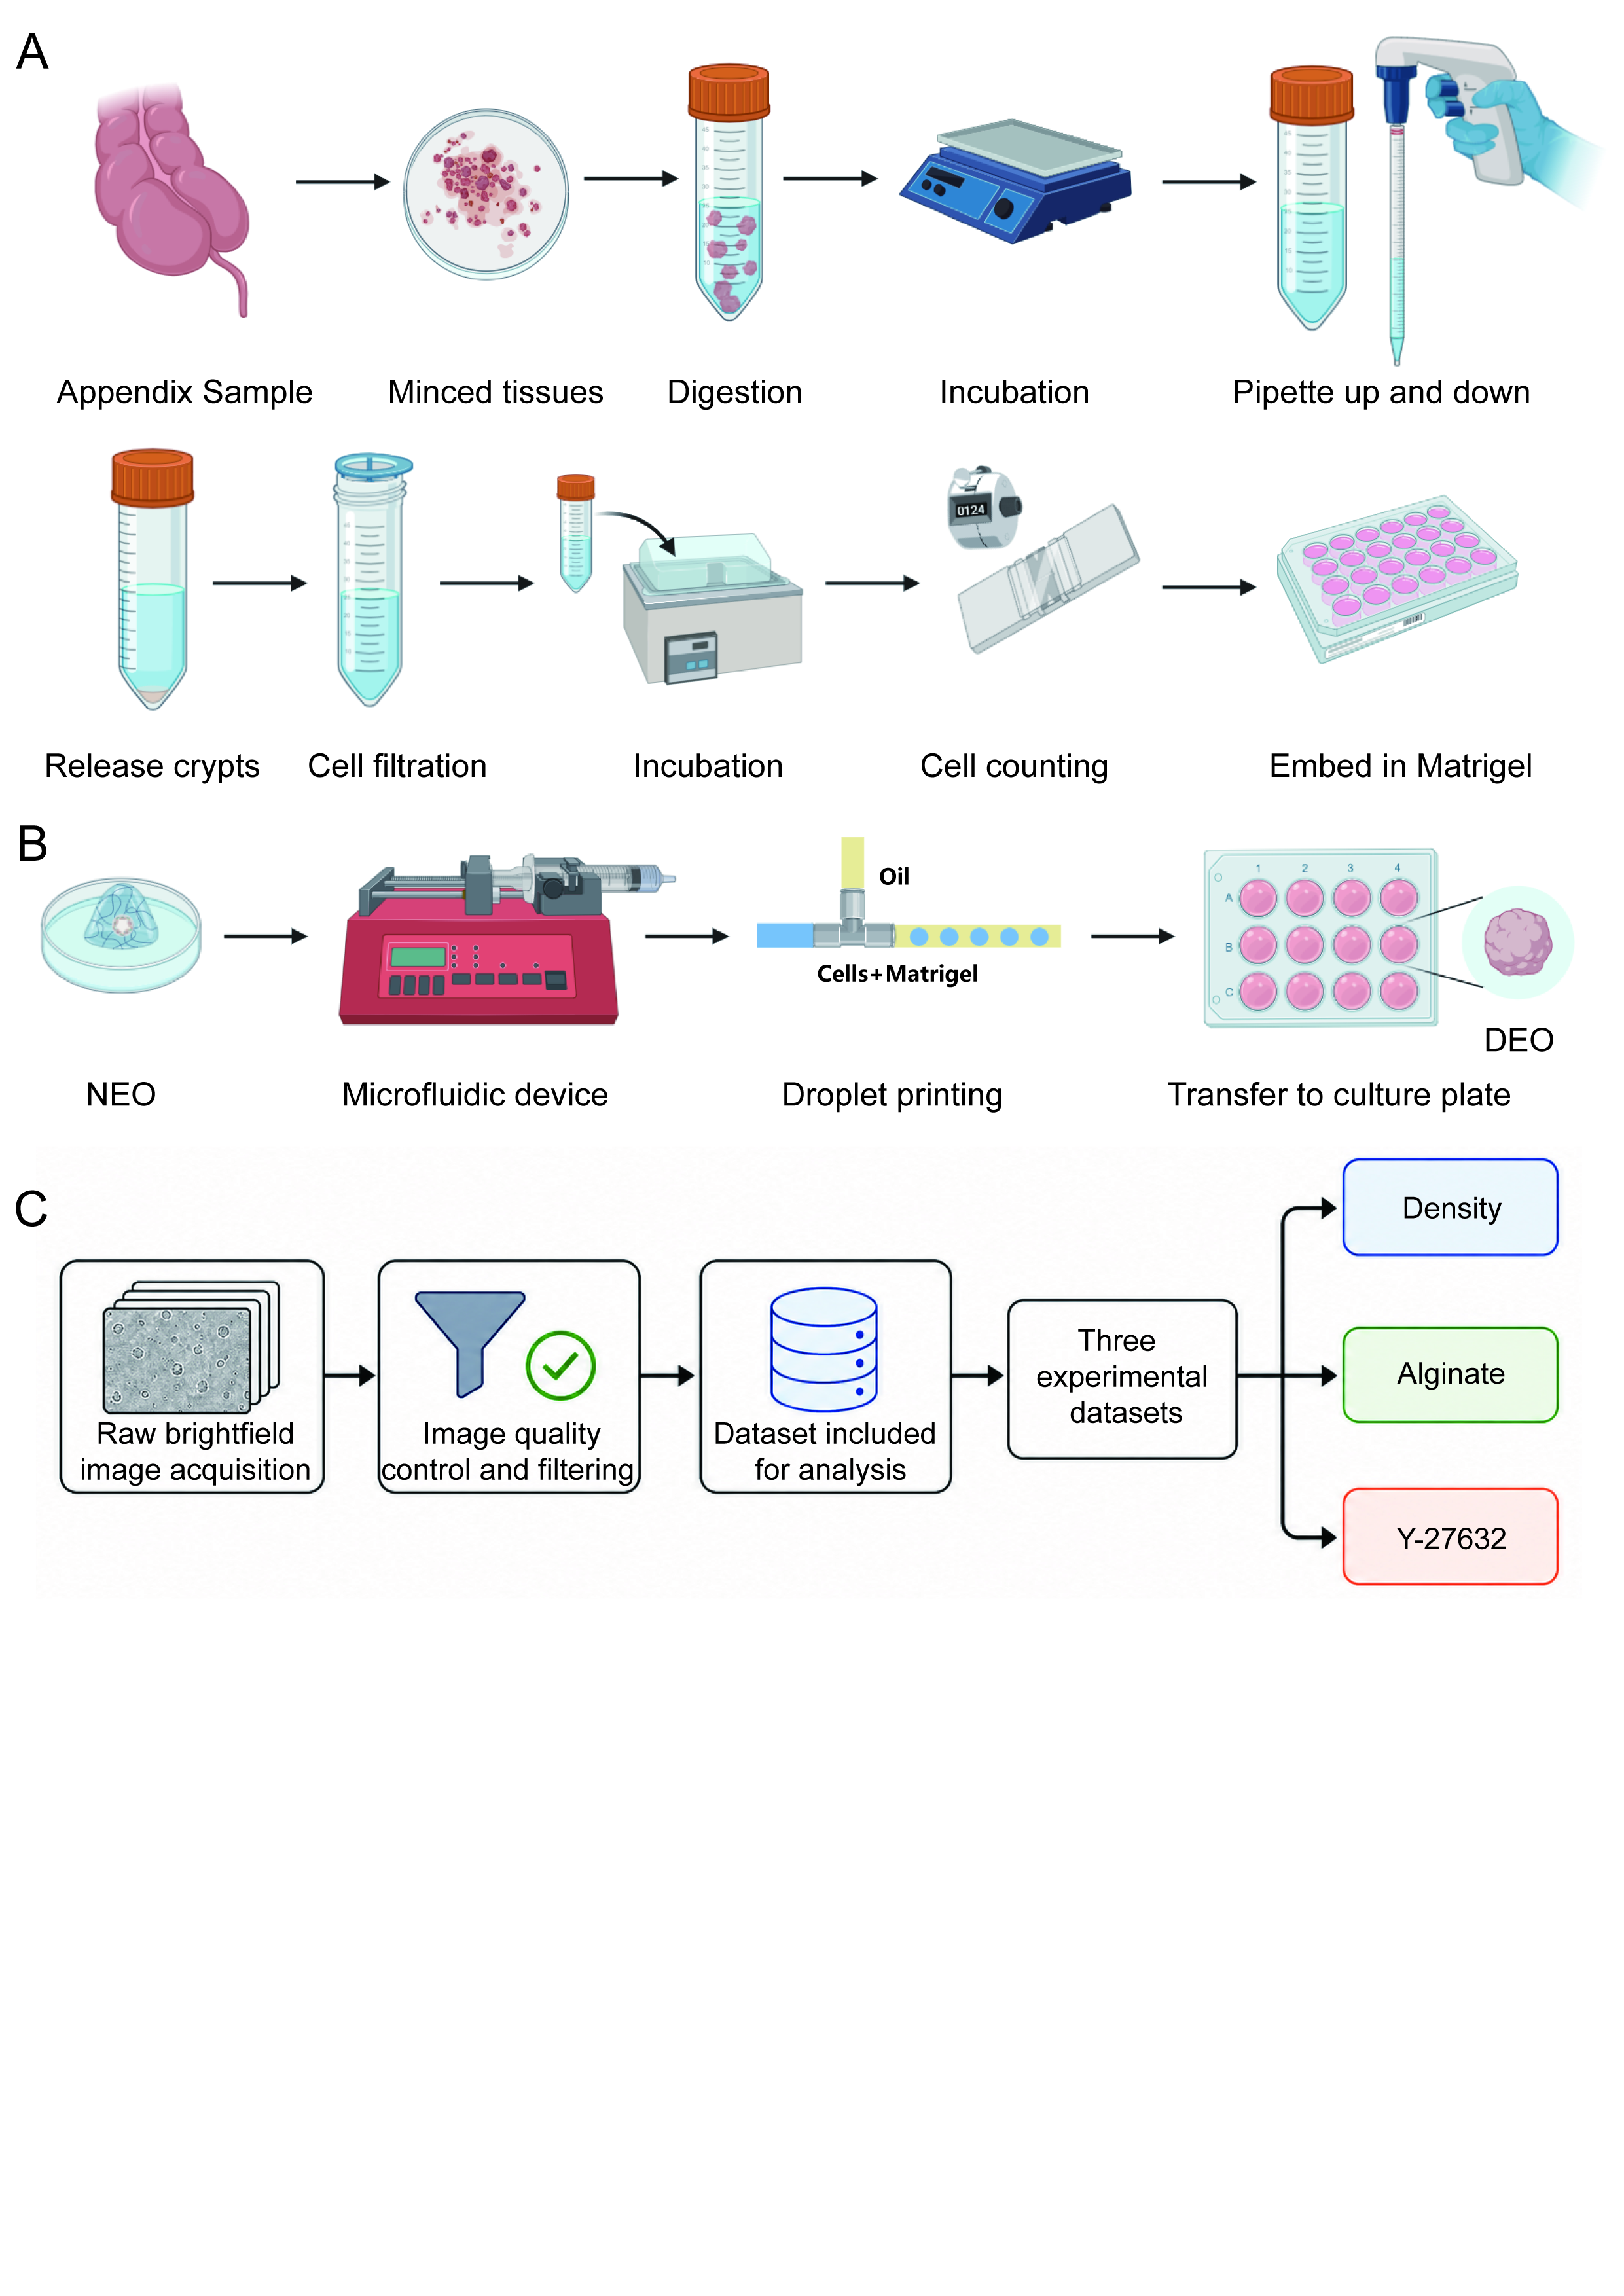
\includegraphics[width=6.36979in,height=6.28646in]{figures/main_figure_01.png}

Figure 1. Schematic overview of establishment of appendix-derived organoids and droplet-engineered organoid (DEO) platform. (A) Schematic diagram of establishment of appendix-derived organoids from human tissues. (B) Schematic illustration of DEO generation from appendix-derived organoids. (C) Dataset management workflow for DEO brightfield image analysis.

替换DEO图片 第一个图增加构建数据集的加入C

附件里把图像的所有panel 弄一个数据集

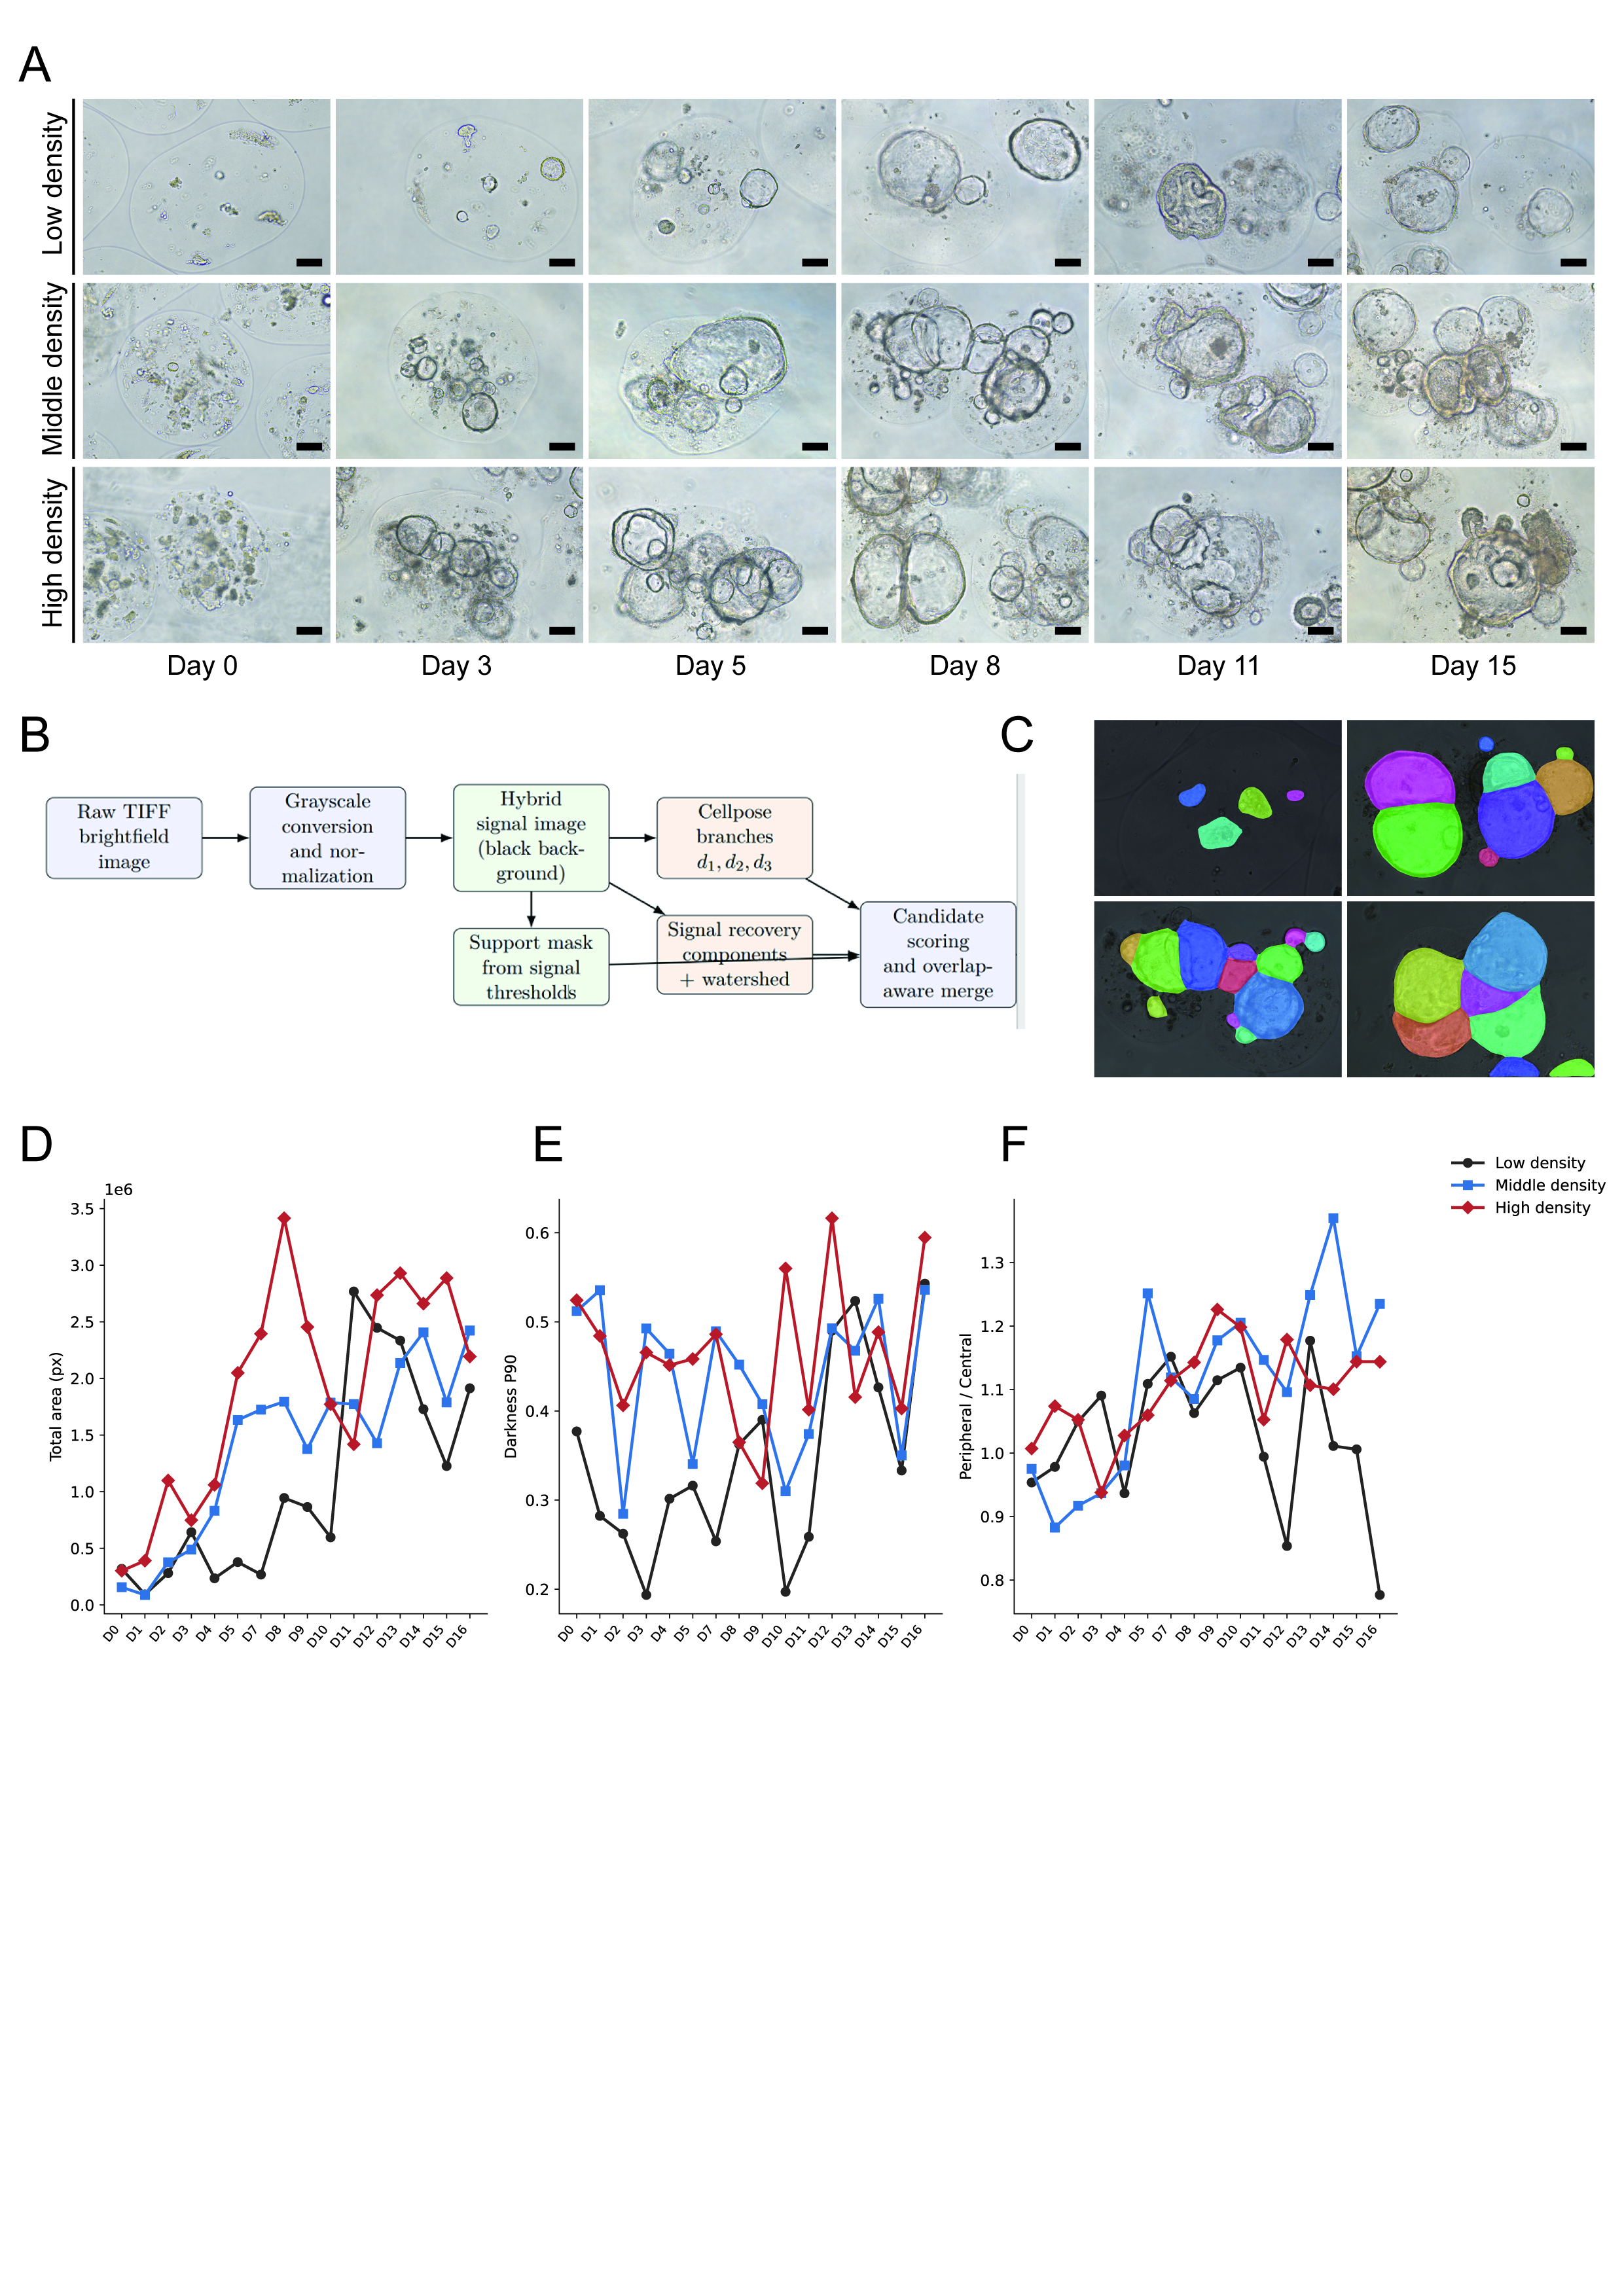
\includegraphics[width=6.36458in,height=6.40069in]{figures/main_figure_02.png}

Figure 2. Effects of initial cell density on the growth of DEOs. (A) Representative brightfield images showing longitudinal development of low, middle, and high density DEOs from day 0 to day15. (B-D) Quantification of growth dynamics (B), differentiation(C), and fusion (D). Scale bars are 100 μm.

\textbf{图的大小一致,字体调整对应 Arial 12号字体，legend单独一个文件，不放在图里}

\textbf{图2是整个AI的agent分割定量以及代表性分割结果}

\textbf{图3-6 可以沿用原来的生物学结果图片以及定量的结果}

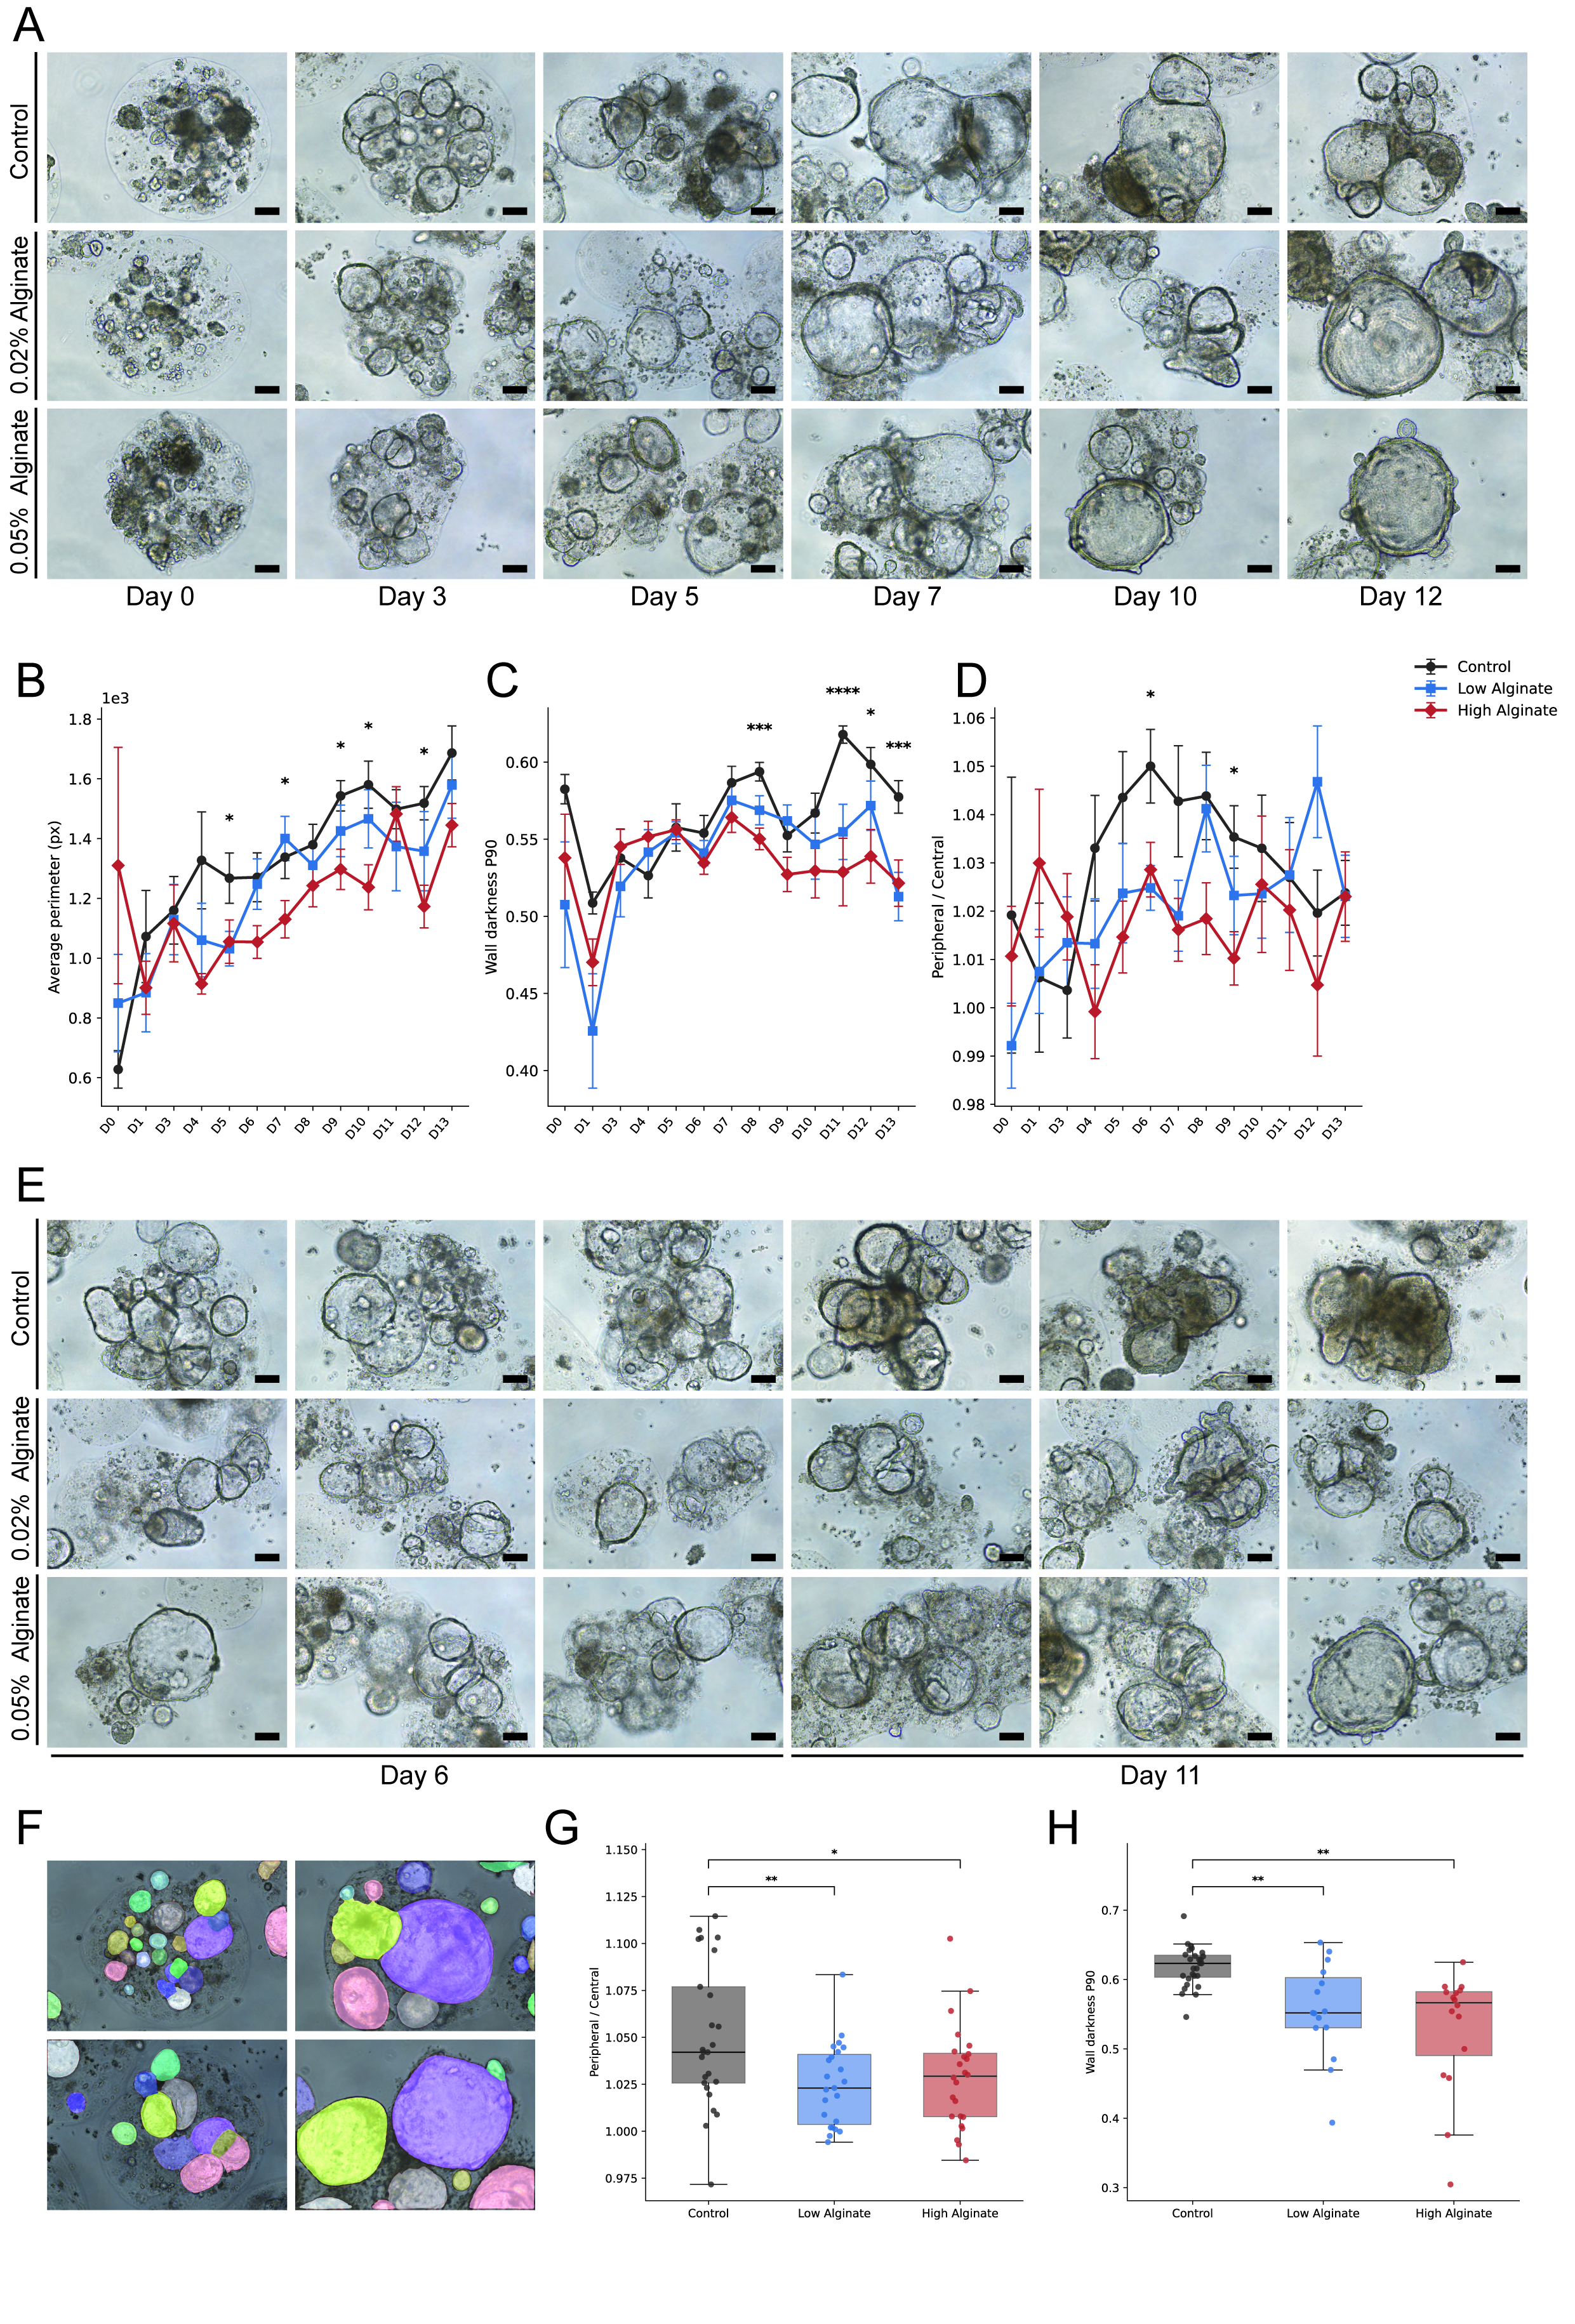
\includegraphics[width=6.08333in,height=8.66146in]{figures/main_figure_03.png}

Figure 3. Alginate incorporation DEOs delayed differentiation. (A) Representative brightfield images of DEOs in Matrigel alone(control) or Matrigel adding sodium alginate at final concentrations of 0.02\% or 0.05\%. Representative images were chosen from day 0 to day 12. (B-D) Quantification of growth dynamics (B), differentiation (C) and fusion behavior (D). Statistical significance was determined by one-way ANOVA followed by a multiple-comparisons test: *P \textless{} 0.05, **P \textless{} 0.01, ***P \textless{} 0.001 and ****P \textless{} 0.0001. Error bars represent mean ± SD. (E) Representative picture at day 6 showing fusion and day 11 showing differentiation during culture. (F-G) Quantification of fusion on day 6 (F) and differentiation on day 11 (G). Statistical significance was determined by one-way ANOVA followed by a multiple-comparisons test: *P \textless{} 0.05, **P \textless{} 0.01. Scale bars are 100 μm.

纵坐标要有单位

\textbf{图的大小一致,字体调整对应 Arial 12号字体，legend单独一个文件，不放在图里}

不要写Low 和high alginate，写0.02\%和0.05\%

把low替换成0.02\%，high 替换成0.05\%

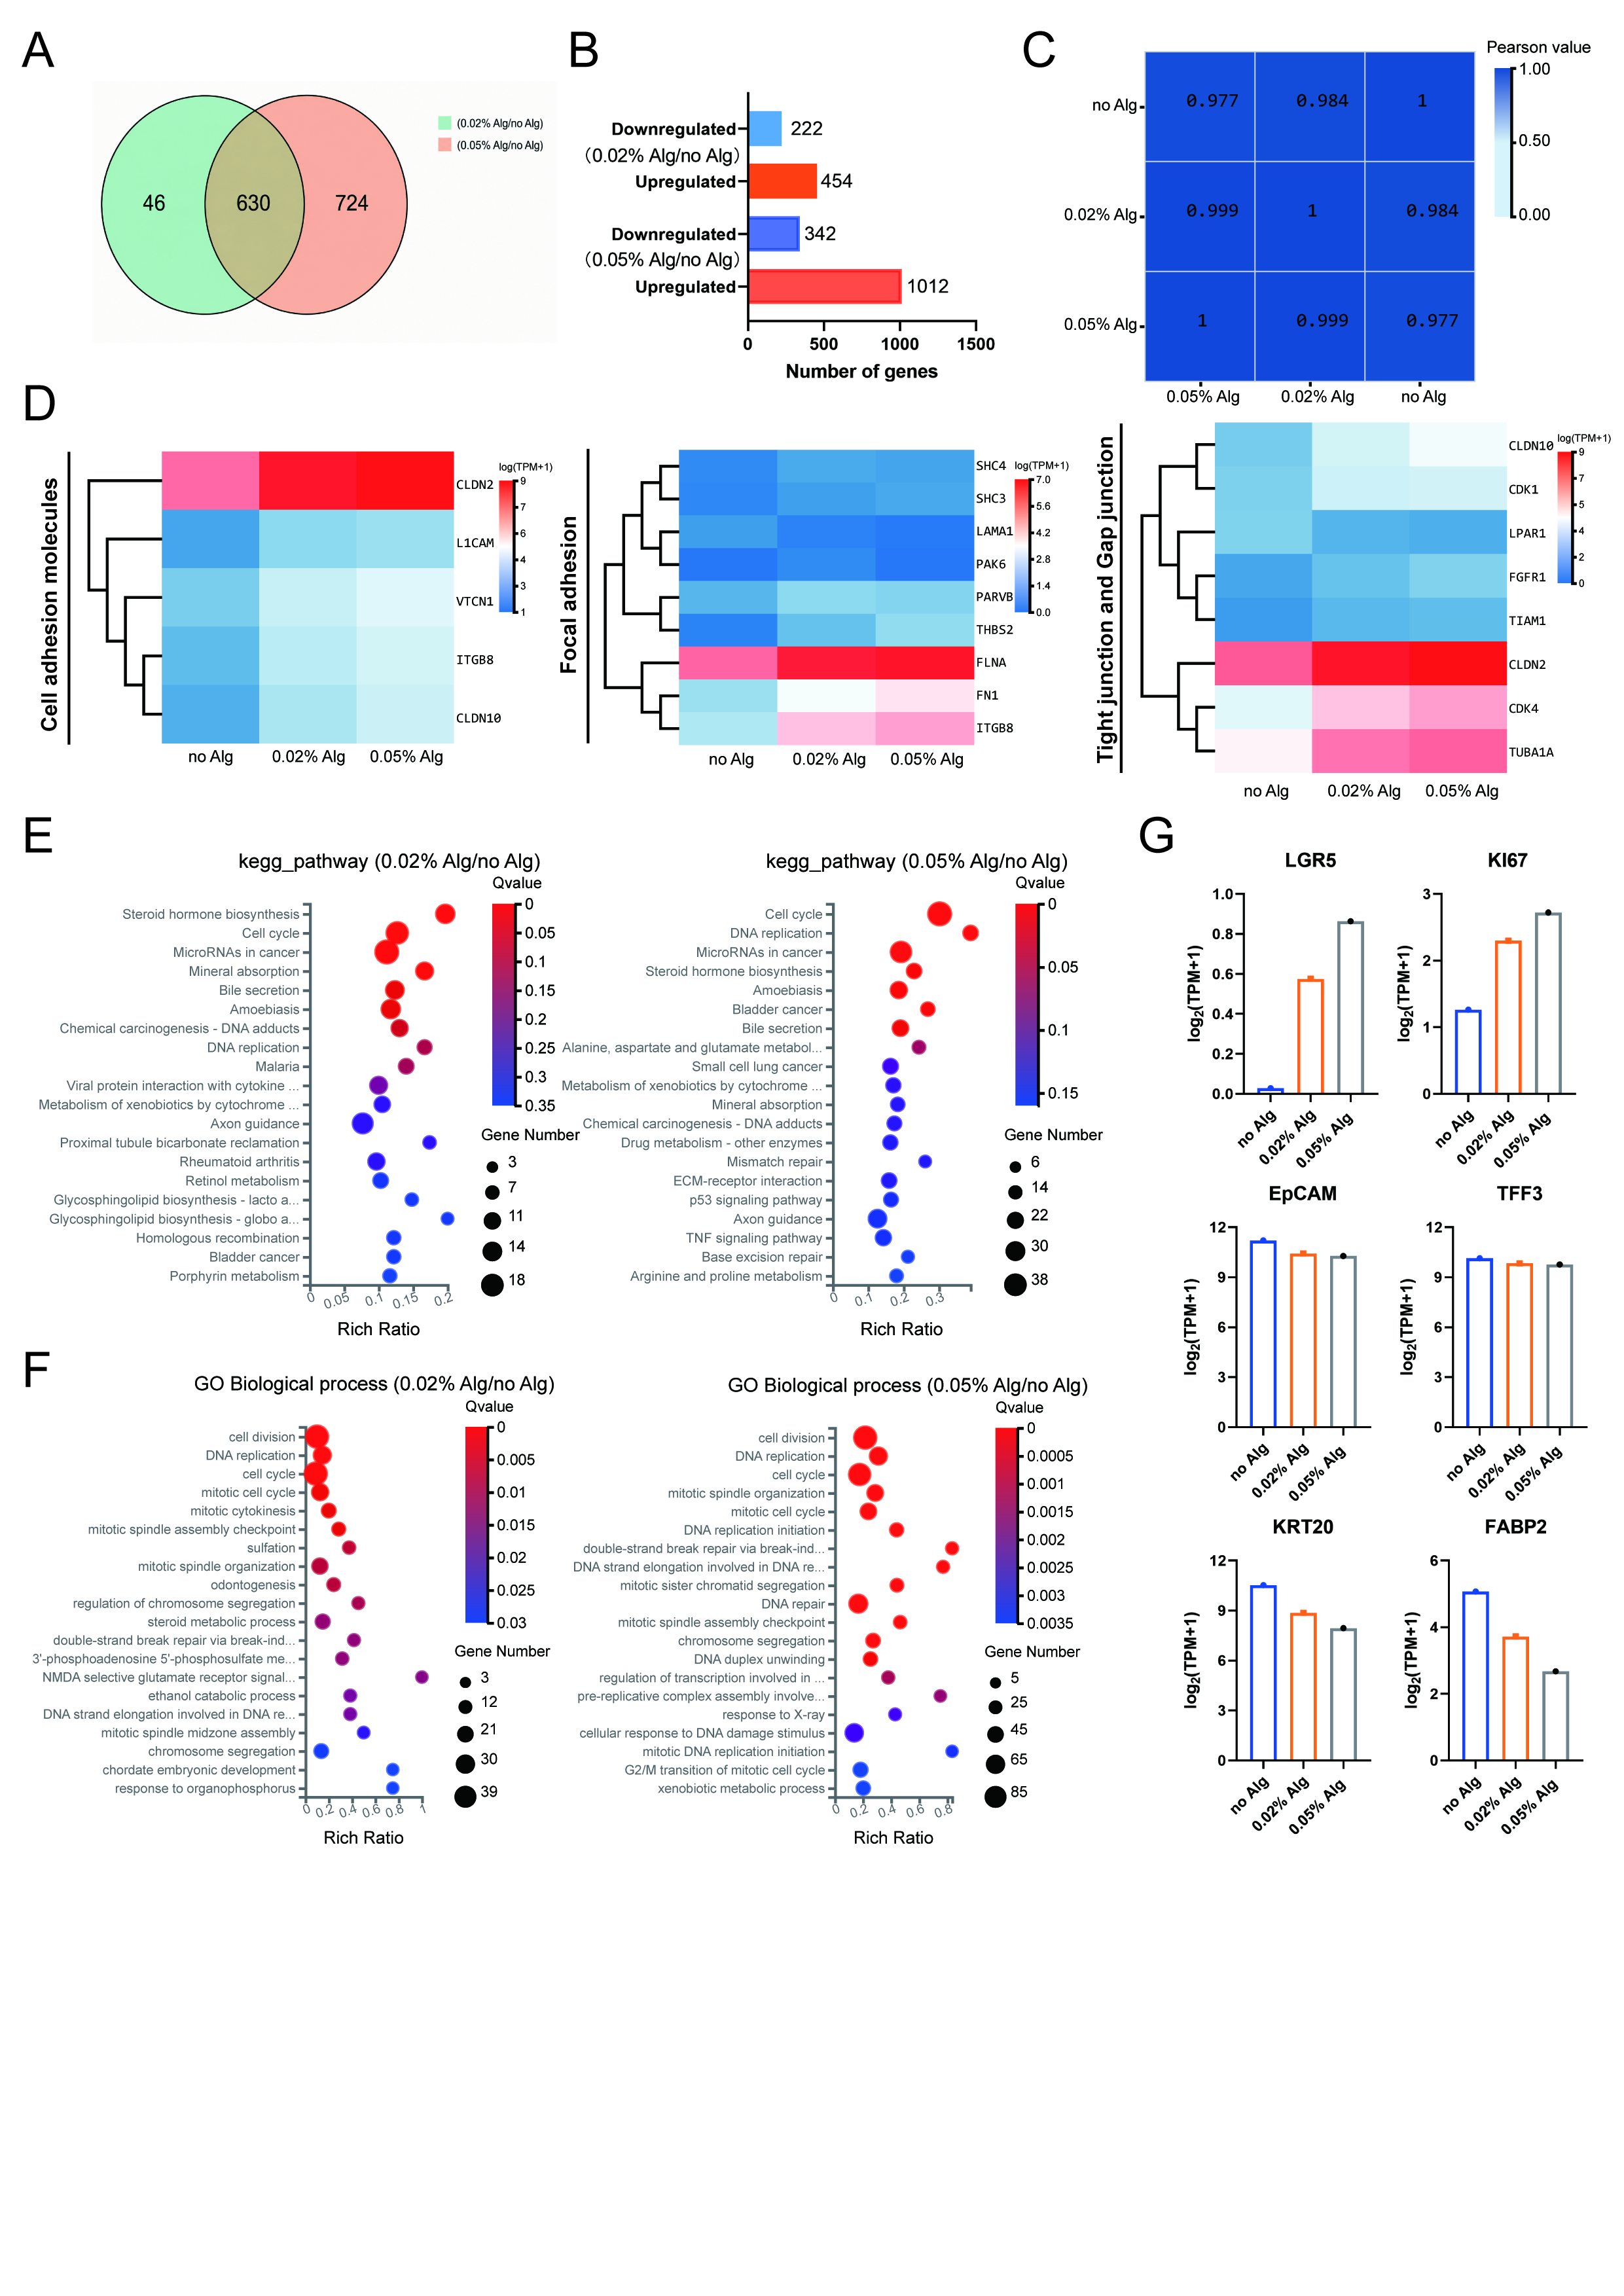
\includegraphics[width=6.36458in,height=7.28125in]{figures/main_figure_04.png}

Figure 4. Transcriptomic analysis of DEOs cultured with or without alginate. (A) Venn diagram showing the overlap of DEGs between 0.02\% alg/no alg and 0.05\% alg/no alg. (B) Bar plots showed the number of upregulated and downregulated DEGs identified in 0.02\% alg/no alg and 0.05\% alg/no alg groups. (C) Pearson correlation heatmap among RNA-Seq samples. (D) Heatmap of DEGs associated with pathways including cell adhesion molecules pathway (KEGG 04514), focal adhesion (KEGG 04510), tight junction (KEGG 04540) and gap junction (KEGG 04520) pathways. (E) Kyoto Encyclopedia of Genes and Genomes (KEGG) pathway enrichment analysis of DEGs between 0.02\% alg/no alg and 0.05\% alg/no alg groups. (F) Gene Ontology Biological Process (GOBP) enrichment analysis of DEGs between 0.02\% alg/no alg and 0.05\% alg/no alg groups. (G) Expression analysis of representative differentiation-related marker genes, including LGR5, KI67, EpCAM, TFF3, KRT20, and FABP2. TPM, transcripts per million.

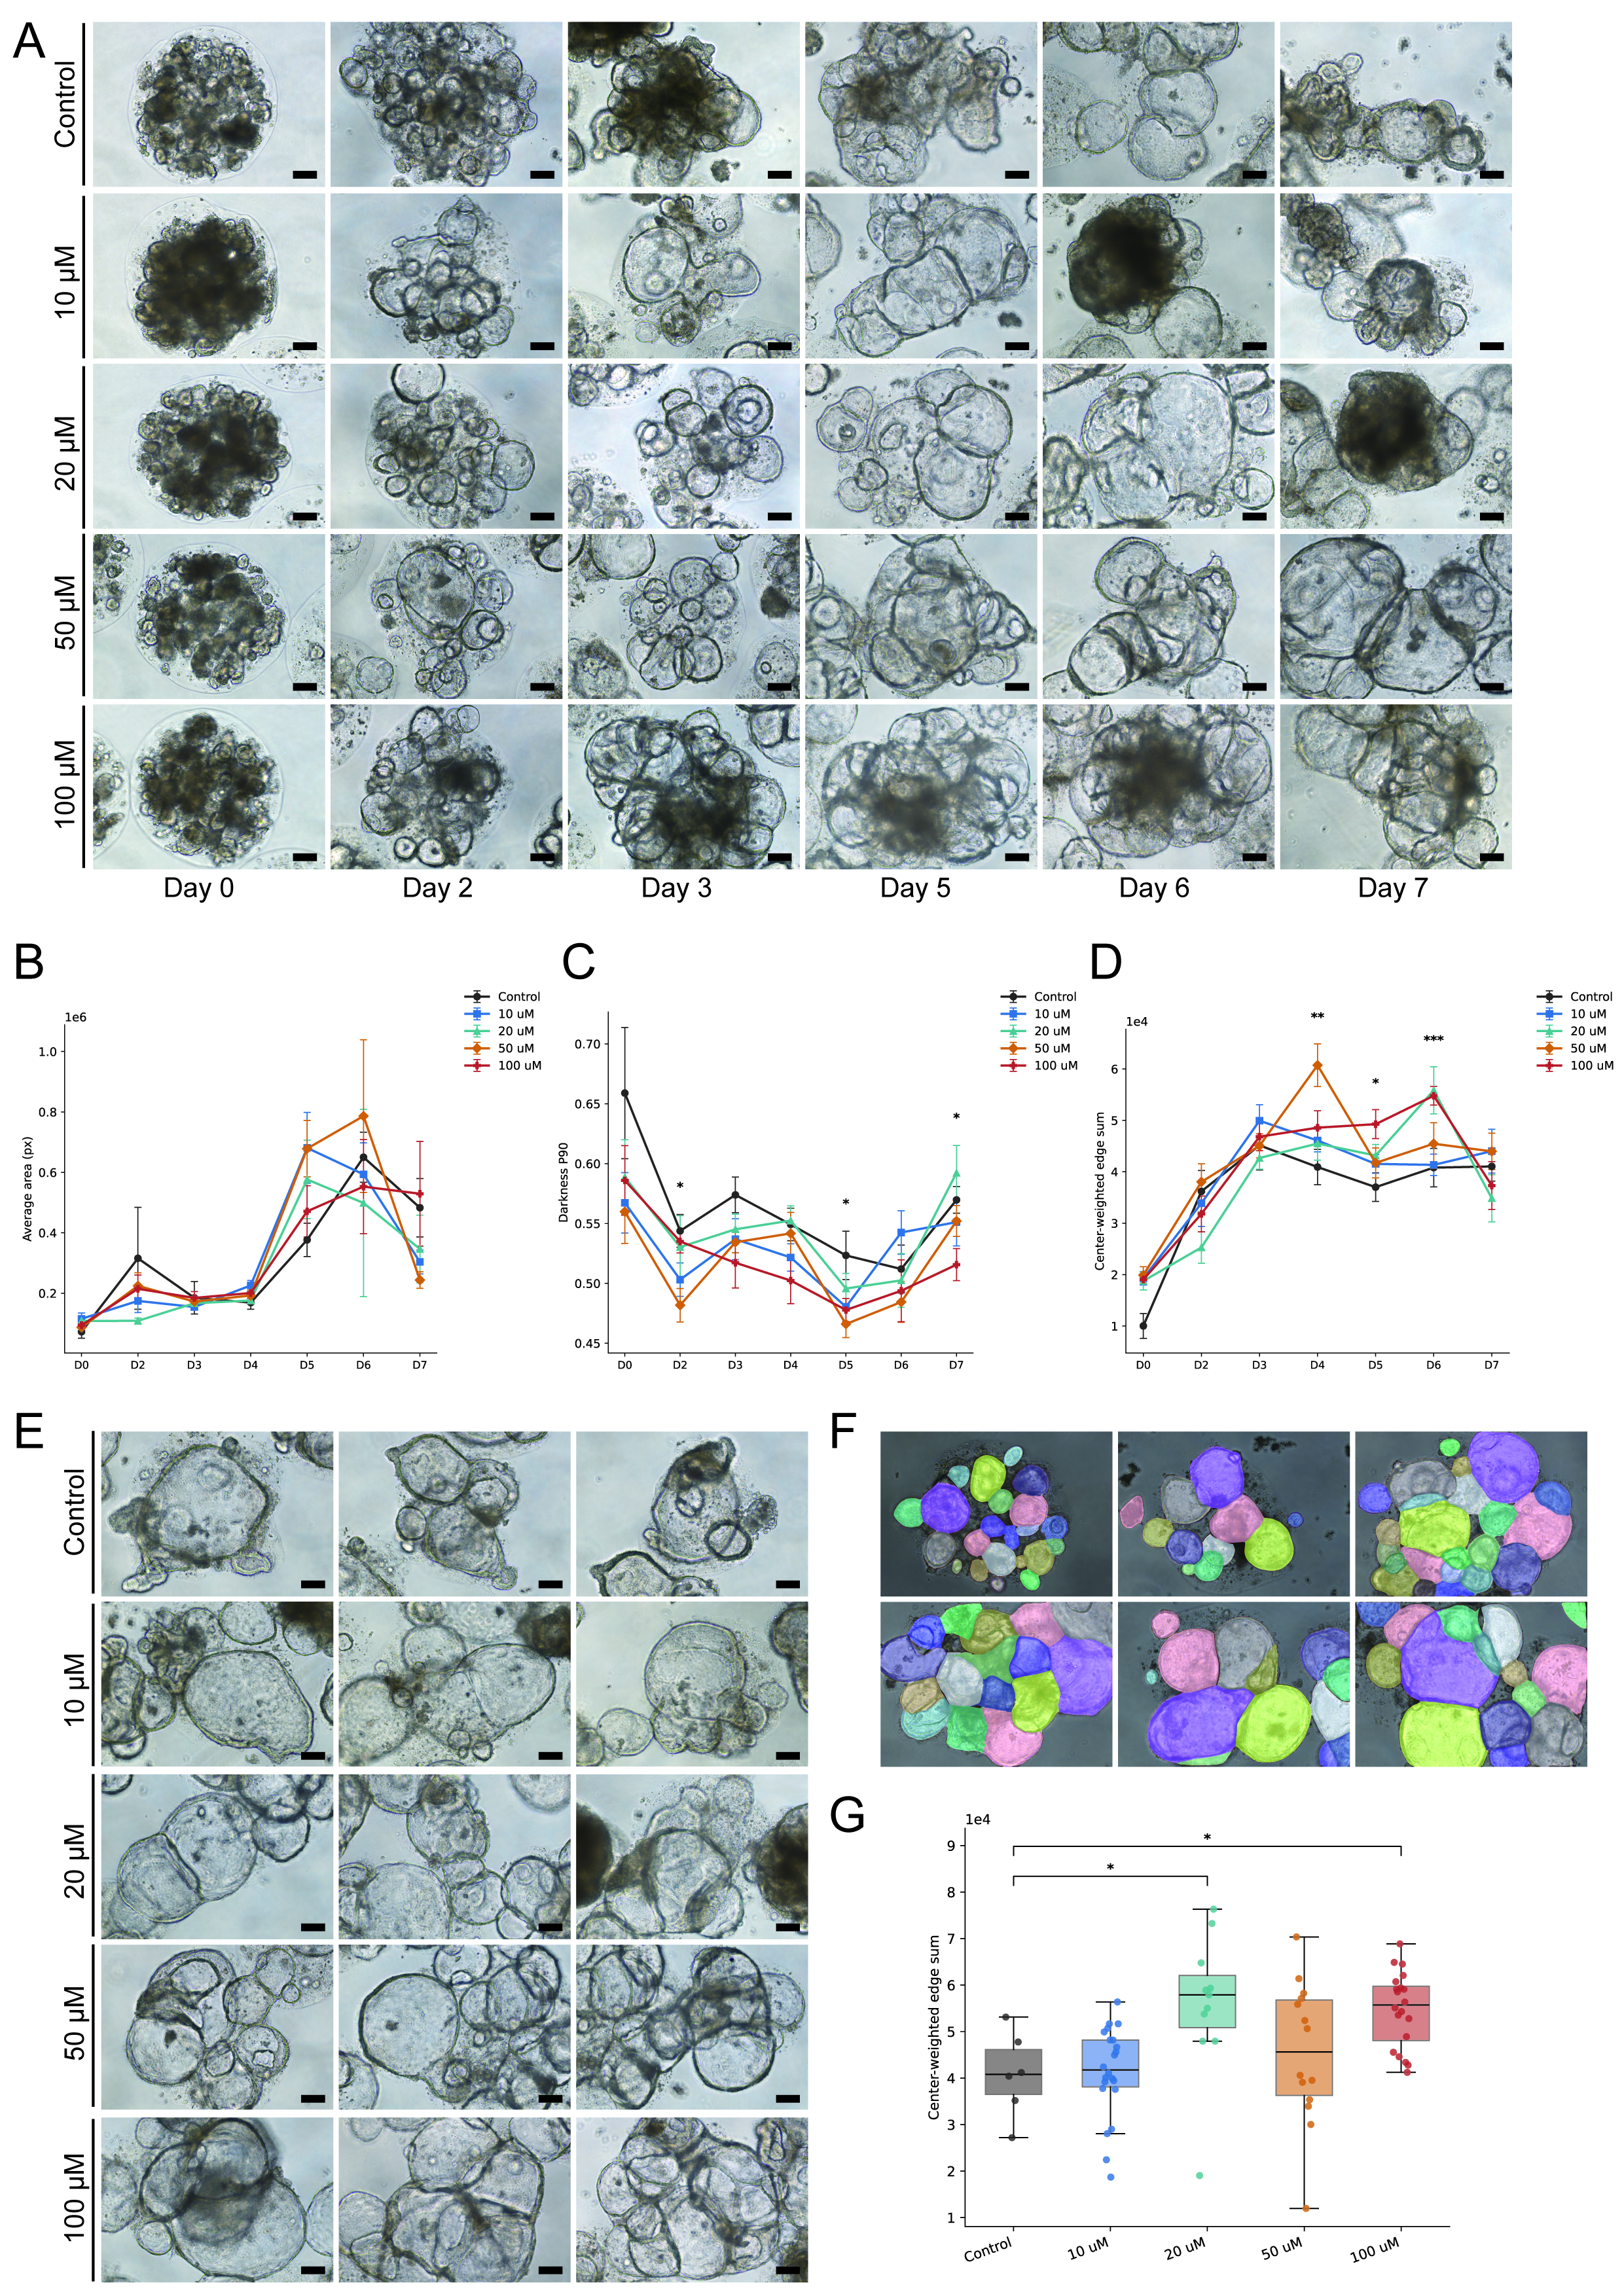
\includegraphics[width=6.36458in,height=9in]{figures/main_figure_05.png}

Figure 5. ROCK inhibition with Y-27632 enhances DEO fusion efficiency and preserves cystic morphology. (A) Representative brightfield images across Y-27632 concentrations from day 0 to day 7. (B-D) Quantification of growth dynamics (B), differentiation (C) and fusion behavior (D). Statistical significance was determined by one-way ANOVA followed by a multiple-comparisons test: *P \textless{} 0.05, **P \textless{} 0.01, and ***P \textless{} 0.001. Error bars represent mean ± SD. (E) Representative images of DEOs on day 6. (F) Quantification of fusion on day 6. Statistical significance was determined by one-way ANOVA followed by a multiple-comparisons test: *P \textless{} 0.05. Scale bars are 100 μm.

\textbf{Method}

\textbf{Establishment of appendix-derived organoids}

Human appendix tissue samples were collected with informed consent from Zhangzhou Municipal Hospital of Fujian Province. The study was approved by the Ethics Committees of Tsinghua Shenzhen International Graduate School (Refs. 202171 and 202295) and Zhangzhou Municipal Hospital of Fujian Province (Ref. 2022KYB277).

Appendix tissues were processed to isolate epithelial crypts, which were embedded in Matrigel and cultured in organoid growth medium. Established organoids were serially passaged and used as the source material for DEO generation. Briefly, human appendix tissue was opened longitudinally, washed with ice-cold PBS, and the mucosal layer was isolated and minced. Tissue fragments were incubated in Gentle Cell Dissociation Reagent (STEMCELL, 100-0485) for 30 minutes on ice, followed by centrifugation and mechanical dissociation in Dulbecco's modified Eagle medium/F12 medium (Gibco, C11330500BT) containing 1\% Bovine Serum Albumin (Sigma-Aldrich, A1933-100G) to release intestinal crypts. The suspension was filtered through a 70 μm cell strainer, and erythrocytes were removed by red blood cell lysis (BioLegend, 420302). Cells were then collected by centrifugation and counted using Trypan Blue (Sigma-Aldrich, T8154). Crypts were resuspended in DMEM/F-12 containing 1\% BSA, mixed 1:1 with growth factor-reduced Matrigel (Corning, 356231), and plated as 50 μL domes in 24-well plates. After solidification at 37°C, cultures were maintained in Human IntestiCult Organoid Growth Medium (OGM, STEMCELL, 06010) supplemented with 50 µg/mL gentamicin (Gibco, 15750060) and 100 µg/mL Primocin (InvivoGen, ant-pm-05). 10 μM Y-27632 (STEMCELL, 72302) was added during initial establishment of primary cultures to improve cell survival. Medium was changed using complete OGM every 2--3 days.

\textbf{Microfluidic generation of DEOs}

Droplet engineered organoids were generated using a microfluidic droplet formation platform established previously in our laboratory {[}9-11{]}. Briefly, organoid domes were incubated in GCDR on ice for 10minutes. Organoid suspensions were centrifuged at 290 g for 5 minutes. Pelleted organoids were resuspended in DMEM/F-12 containing 1\% BSA and mechanically dissociated into smaller crypts by pipetting up and down. Dissociated organoid cells were resuspended in Matrigel (Corning, 356234) to form the aqueous phase, while Engineered Fluid (3M, Novec 7000) served as the oil phase. The two phases were connected to a custom T-junction PDMS and connected to microfluidic device (lead fluid) through microfluidic PTFE tubing (Woer, 24T). 1 mL syringe was used for aqueous phase and 10 mL syringe for oil phase. The controlled flow conditions were set as oil phase at 140 μL/min and the aqueous phase at 8 μL/min. All reagents and device components for aqueous phase were maintained in 4°C refrigerator throughout droplet generation. Following solidification at 37°C for 30 min, droplets were transferred into OGM and residual oil was removed before plating. The droplets were then maintained in ultra-low-attachment 12 well plates (LV-ULA002-12W) at 37°C 5\% CO\textsubscript{2}. For density experiments, low, middle and high-density suspensions were prepared before droplet generation. Droplet morphology and structural integrity were checked by microscopy.

\textbf{Alginate-based DEO generation}

Alginate-based DEOs were generated using a modified microfluidic protocol adapted from our previous method {[}21{]}. Sodium alginate powder (MACKLIN, S817374) was dissolved in sterile physiological saline to obtain a 1\% (w/v) stock solution, which was subsequently diluted to 0.5\% and 0.2\% (w/v). All alginate solutions were sterilized by passing through 0.22 μm membrane filters. Calcium chloride (CaCl\textsubscript{2}, Sigma-Aldrich, C5670) was dissolved in deionized water to prepare a 1\% (w/v) solution and similarly sterilized by filtration. Microfluidic setup and droplet generation were performed as described for Matrigel-based DEOs with indicated difference in aqueous phase components. Cells were resuspended in cold Matrigel, followed by adding diluted alginate solution to make final alginate concentrations of 0.05\% or 0.02\% (w/v). The cell--matrix mixture was then put into the microfluidic device for droplet generation. After droplet formation, DEOs were incubated at 37°C to let Matrigel solidification. The DEOs were then pumped out of the PTFE tube by using a syringe and immediately transferred into CaCl\textsubscript{2} solution for 5 minutes to induce alginate crosslinking. After crosslinking, DEOs were washed three times using sterile physiological saline to remove excess calcium ions followed by a final wash in Dulbecco's phosphate-buffered saline (DPBS, Servicebio, G4200) and then maintained in complete OGM in ultra-low-attachment 12 well plates until further use. DEOs cultured in Matrigel without alginate served as controls.

\textbf{Y-27632 treatment}

The powder of Y-27632 (STEMCELL, 72302) was resuspended in 624 µL of PBS to make a 5 mM stock solution. Stock solution diluted into 0, 10, 20, 50, or 100 μM Y-27632 culture medium was added to DEOs grown in OGM. Culture medium was carefully removed without interrupting the DEOs, then replenished every 2 days using fresh medium. Morphology and fusion behavior were recorded by brightfield microscopy.

\textbf{RNA sequencing analysis}

Total RNA was extracted from alginate-based DEOs (no-alginate, low-alginate, and high-alginate) using TRIzol reagent (Invitrogen, 15596026) according to the manufacturer's instructions. Organoids were disrupted by repeated pipetting to obtain a homogeneous lysate. RNA quality and concentration were evaluated prior to library construction. Poly(A)+ mRNA libraries were prepared using the mRNA Library Kit (BGI, Shenzhen, China). In brief, mRNA sequencing libraries were constructed using the mRNA Library Kit (BGI, Shenzhen, China). RNA samples were denatured followed by mRNA enrichment using oligo(dT)-conjugated magnetic beads. The enriched mRNA was then fragmented. First-strand cDNA synthesis was performed with random hexamer primers, and second-strand cDNA was subsequently synthesized to generate double-stranded cDNA. After that, the cDNA underwent end repair, and a single deoxyadenosine (A) nucleotide was added to the 3' ends of the blunt-ended fragments. The adaptors were ligated to the A-tailed cDNA, and the final library was amplified by PCR. And the final PCR products were circularized to form single-stranded DNA circles. After digesting linear molecules, the circularized DNA underwent rolling circle amplification (RCA) to produce DNA nanoballs (DNBs). Finally, the DNBs needed to load into a patterned nanoarray and sequenced on the DNBSEQ platform to generate PE150 bases reads. Later RNA-seq data processing and analysis were conducted using an integrated RNA-seq analysis system Dr. Tom platform provided by BGI.

\textbf{AAPS Organoid Agent for image segmentation and quantitative morphology}

Brightfield image analysis was implemented as a harnessed AAPS Organoid Agent workflow rather than a single fixed segmentation script. The goal of the harness was to make agentic image analysis reproducible: each run registered the source image path, experiment branch, date, condition or concentration, replicate, magnification, output mask, overlay, metric JSON, and summary CSV in a persistent file database. The final analysis roots were app81\_density\_stitched\_cellpose\_v5\_final\_metrics\_v1 for density experiments, app65\_alginate\_v3\_direct\_brightfield for alginate experiments, and app80\_all\_concentrations\_multiscale\_large\_recovery for Y-27632 experiments. The database layer included source\_image\_database.csv, per-image metric tables, daily summary tables, and manifest files. The AAPS harness therefore separated the biological experiment design from low-level image-processing choices and preserved the provenance required to audit each final measurement.

The AAPS workflow followed a register-inspect-route-segment-verify-quantify pattern. First, images were registered from the raw experiment folders and converted into a canonical metadata table. Second, the image was inspected for modality, magnification, object density, expected object scale, and image quality. Third, the harness routed the image to the most appropriate segmentation branch. This routing was necessary because the three experiments had different image priors: density images contained stitched 10× panels with variable organoid counts, alginate images included many directly acquired brightfield fields, and Y-27632 images contained concentration-dependent large fused organoids. The final segmentation branch could therefore combine multiscale Cellpose, deterministic thresholding, signal-based large-object recovery, and, for selected difficult App81 panels, image-generation-assisted mask refinement using Nano Banana 2.

For deterministic preprocessing, each raw TIFF image was converted to an 8-bit grayscale image \(I\left( x \right)\). Contrast-limited adaptive histogram equalization was applied, followed by a small Gaussian blur \(F\left( x \right)\) and a larger background blur \(B\left( x \right)\). The AAPS signal image was defined as a weighted combination of inverted foreground intensity and background-subtracted residual:

\[S\left( x \right) = 0.45\,\text{norm}\left( 255 - F\left( x \right) \right) + 0.55\,\text{norm}\left( B\left( x \right) - F\left( x \right) \right)\]

where \(\text{norm}\left( \cdot \right)\) denotes min--max normalization to 0--255. A support mask was generated by combining Otsu thresholding with a percentile floor:

\[T_{\sup} = max\{ T_{\text{Otsu}}\left( S \right),Q_{0.58}\left( S \right)\}\]

\[M_{\sup}\left( x \right) = \mathbf{1}\left\lbrack S\left( x \right) \geq T_{\sup} \right\rbrack\]

followed by morphological opening and closing. This support mask was not treated as the final segmentation; it served as an image prior for candidate filtering, large-object recovery, and quality control.

For multiscale instance segmentation, Cellpose was run at several candidate diameters instead of assuming one organoid size. App65 used a direct brightfield branch with diameters of 220, 320, 420, 520, and 700 pixels. App80 used date- and morphology-aware diameter schedules, with larger diameters routed to later fused stages. App81 density images were first analyzed as stitched 3 × 3 collages to exploit repeated panel context; multiple Cellpose diameter settings were tested, and selected panel-level outputs from 1×, 2×, and 4× diameter runs were merged when one setting better recovered a local field. Candidate objects from Cellpose and signal-threshold recovery were scored by support overlap, mean signal, edge strength, fill ratio, size, and stage prior. Overlapping candidates were merged using overlap-aware rules based on intersection-over-union and overlap over the smaller mask. The final output for each image was an integer instance label image \(L\left( x \right) \in \{ 0,1,\ldots,K\}\), with zero denoting background and labels \(1,\ldots,K\) denoting organoid instances.

For App81 density data, the AAPS harness included a human-in-the-loop quality-control step because several stitched panels contained large organoids that were missed by the most stable Cellpose setting. In these selected panels, Nano Banana 2 was provided with the original stitched image and the current Cellpose color-mask overlay, then prompted to preserve the existing correct segmentation while adding or correcting the missed organoid instance. The generated masks were not accepted automatically. They were visually reviewed, merged only into targeted panels, exported back from stitched coordinates to single-image masks, and then backfilled into the same per-image database as the pure Cellpose outputs. In the final App81 metric table, 63 canonical source images were retained and 49 duplicate exports were ignored by the database backfill step.

\textbf{AAPS metric design and mathematical definitions}

Metric selection was performed by the AAPS Organoid Agent using the experiment design and then finalized by human-in-the-loop review. The agent selected one primary growth, differentiation, and fusion readout per experiment, while also retaining auxiliary metrics for audit and sensitivity checks. Let \(\Omega\) be the image domain and let \(\Omega_{k} = \{ x:L\left( x \right) = k\}\) be organoid instance \(k\). Let \(A_{k} = \left| \Omega_{k} \right|\), \(P_{k}\) be its perimeter, and \(K\) be the instance count. The total segmented area and mean instance area were defined as

\[A_{\text{tot}} = \sum_{k = 1}^{K}A_{k},\text{\quad\quad}\bar{A} = K^{- 1}\sum_{k = 1}^{K}A_{k}\]

and the mean perimeter was

\[\bar{P} = K^{- 1}\sum_{k = 1}^{K}P_{k}\]

The density experiment used \(A_{\text{tot}}\) as the growth readout because the biological question concerned total organoid expansion within each droplet field. The alginate experiment used \(\bar{P}\) because perimeter was more sensitive to morphology and epithelial expansion under matrix modification. The Y-27632 experiment used \(\bar{A}\) because fusion changed object number and total area alone could confound growth with fusion-associated merging.

Differentiation-like morphology was quantified using darkness metrics designed to capture dark, thickened, or budded epithelial structures. A background median \(b\) was estimated from the complement of a dilated union mask. Pixel darkness was defined as

\[D\left( x \right) = clip\left( \frac{b - I\left( x \right)}{\max\left( b,1 \right)},0,1 \right)\]

Organoid darkness P90 was the 90th percentile of \(D\left( x \right)\) over all segmented organoid pixels. For wall-specific darkness, each instance was split into an adaptive wall and core. The equivalent radius was \(r_{k} = \sqrt{A_{k}/\pi}\), the wall thickness was \(t_{k} = clip\left( \text{round}\left( 0.12r_{k} \right),5,30 \right)\) pixels, and the core was obtained by eroding \(\Omega_{k}\) by \(t_{k}\). Wall darkness P90 was the 90th percentile of \(D\left( x \right)\) over the wall pixels. Density and Y-27632 experiments used organoid darkness P90, whereas the alginate experiment used wall darkness P90 to emphasize epithelial wall thickening.

Fusion metrics were based on the premise that organoid fusion redistributes edge structure from object peripheries toward the interior of large integrated masses. For each instance, a normalized centrality field was computed from the distance transform:

\[C_{k}\left( x \right) = \frac{\text{dist}\left( x,\partial\Omega_{k} \right)}{\max_{y \in \Omega_{k}}\text{dist}\left( y,\partial\Omega_{k} \right)}\]

Let \(E\left( x \right)\) denote the normalized internal edge or hybrid-signal edge field. Central and peripheral internal edge means were

\[E_{\text{cen}} = \frac{\sum_{k}^{}{\sum_{x \in \Omega_{k}}^{}E}\left( x \right)C_{k}\left( x \right)}{\sum_{k}^{}{\sum_{x \in \Omega_{k}}^{}C_{k}}\left( x \right)}\]

\[E_{\text{per}} = \frac{\sum_{k}^{}{\sum_{x \in \Omega_{k}}^{}E}\left( x \right)\left( 1 - C_{k}\left( x \right) \right)}{\sum_{k}^{}{\sum_{x \in \Omega_{k}}^{}\left( 1 - C_{k}\left( x \right) \right)}}\]

The peripheral-to-central ratio was

\[R_{per/cen} = \frac{E_{\text{per}}}{E_{\text{cen}}}\]

and was used for density and alginate experiments because it directly reports peripheral versus interior edge redistribution. For the Y-27632 experiment, the primary fusion readout was a center-weighted edge sum:

\[S_{\text{cw}} = \sum_{k = 1}^{K}{\sum_{x \in \Omega_{k}}^{}E}\left( x \right)\frac{\exp\left( 5C_{k}\left( x \right) \right) - 1}{\exp\left( 5 \right) - 1}\]

which emphasizes internal edges in fused structures and was more suitable for ROCK-inhibition-induced structural integration.

All final primary and auxiliary metrics were written at per-image resolution and then summarized by condition and date. App81 density outputs included 63 canonical images; App65 alginate outputs included 886 images; and App80 Y-27632 outputs included 646 images. The AAPS harness stored masks, random-color instance maps, overlays, signal images, metric JSON files, per-image CSV files, daily summaries, figure outputs, and manifests. This allowed large batches to be processed dynamically while preserving human-in-the-loop checkpoints for segmentation review, prompt-guided correction, metric selection, and final figure generation. Representative segmentation outputs for the density, alginate, and Y-27632 experiments are shown in Figures S4, S5, and S6, respectively, and the primary metric choices are summarized in Table S1.

\textbf{Statistical analysis}

Statistical analyses were performed as follows. Normality of data distribution was first assessed for each dataset using the Shapiro-Wilk test. For comparisons among multiple groups at individual time points, normally distributed data was analyzed by one-way ANOVA followed by Dunnett's multiple-comparisons test against the control group. Data are presented as mean ± SD unless otherwise indicated. Statistical significance was defined as probability (P) value of less than 0.05. Significant differences are shown in the figures as follows: *P \textless{} 0.05, **P \textless{} 0.01, ***P \textless{} 0.001 and ****P \textless{} 0.001.

\textbf{Acknowledgments}

The work was supported by XXXX.

\textbf{Author Contribution}

Z.W. contributed to conceptualization, methodology, data analysis, visualization, and writing of the original draft. R.C. contributed to brightfield image quantification，AAPS Organoid Agent. W.W. participated in experiments involving alginate-containing production. C.R. and H.S. provided experimental materials and technical support. S.M. supervised the study, provided administrative support, and acquired funding. All authors reviewed and edited the manuscript and contributed to the revision process.

\textbf{Data availability}

The data supporting the results of this study can be obtained from the corresponding author upon reasonable request.

\textbf{References}

1. Almeqdadi, M., et al., \emph{Gut organoids: mini-tissues in culture to study intestinal physiology and disease.} Am J Physiol Cell Physiol, 2019. \textbf{317}(3): p. C405-c419.2. Corrò, C., L. Novellasdemunt, and V.S.W. Li, \emph{A brief history of organoids.} Am J Physiol Cell Physiol, 2020. \textbf{319}(1): p. C151-c165.3. Dedhia, P.H., et al., \emph{Organoid Models of Human Gastrointestinal Development and~Disease.} Gastroenterology, 2016. \textbf{150}(5): p. 1098-1112.4. Günther, C., et al., \emph{Organoids in gastrointestinal diseases: from experimental models to clinical translation.} Gut, 2022. \textbf{71}(9): p. 1892-1908.5. Taelman, J., M. Diaz, and J. Guiu, \emph{Human Intestinal Organoids: Promise and Challenge.} Front Cell Dev Biol, 2022. \textbf{10}: p. 854740.6. Zhao, Z., et al., \emph{Organoids.} Nat Rev Methods Primers, 2022. \textbf{2}.7. Phipson, B., et al., \emph{Evaluation of variability in human kidney organoids.} Nat Methods, 2019. \textbf{16}(1): p. 79-87.8. Rosenbluth, J.M., et al., \emph{Organoid cultures from normal and cancer-prone human breast tissues preserve complex epithelial lineages.} Nat Commun, 2020. \textbf{11}(1): p. 1711.9. Jiang, S., et al., \emph{An Automated Organoid Platform with Inter-organoid Homogeneity and Inter-patient Heterogeneity.} Cell Rep Med, 2020. \textbf{1}(9): p. 100161.10. Li, J., et al., \emph{Microdroplet-Engineered Skeletal Muscle Organoids from Primary Tissue Recapitulate Parental Physiology with High Reproducibility.} Research (Wash D C), 2025. \textbf{8}: p. 0699.11. Yang, H., et al., \emph{Ultra-small tissue-compatible organoid printer for rapid and controllable modeling of respiratory organoids.} Device, 2024. \textbf{2}(8): p. 100420.12. Orkin, R.W., et al., \emph{A murine tumor producing a matrix of basement membrane.} J Exp Med, 1977. \textbf{145}(1): p. 204-20.13. Fujii, M., et al., \emph{Human Intestinal Organoids Maintain Self-Renewal Capacity and Cellular Diversity in Niche-Inspired Culture Condition.} Cell Stem Cell, 2018. \textbf{23}(6): p. 787-793.e6.14. Sachs, N., et al., \emph{Intestinal epithelial organoids fuse to form self-organizing tubes in floating collagen gels.} Development, 2017. \textbf{144}(6): p. 1107-1112.15. Sato, T., et al., \emph{Single Lgr5 stem cells build crypt-villus structures in vitro without a mesenchymal niche.} Nature, 2009. \textbf{459}(7244): p. 262-5.16. Zhao, H., et al., \emph{Droplet-engineered organoids recapitulate parental tissue transcriptome with inter-organoid homogeneity and inter-tumor cell heterogeneity.} Fundam Res, 2024. \textbf{4}(6): p. 1506-1514.17. Francis, K. and B.O. Palsson, \emph{Effective intercellular communication distances are determined by the relative time constants for cyto/chemokine secretion and diffusion.} Proc Natl Acad Sci U S A, 1997. \textbf{94}(23): p. 12258-62.18. Hofer, M. and M.P. Lutolf, \emph{Engineering organoids.} Nat Rev Mater, 2021. \textbf{6}(5): p. 402-420.19. Capeling, M.M., et al., \emph{Nonadhesive Alginate Hydrogels Support Growth of Pluripotent Stem Cell-Derived Intestinal Organoids.} Stem Cell Reports, 2019. \textbf{12}(2): p. 381-394.20. Tang, X., et al., \emph{Volumetric compression by heterogeneous scaffold embedding promotes cerebral organoid maturation and does not impede growth.} Cell Syst, 2023. \textbf{14}(10): p. 872-882.e3.21. Wang, Z., et al., \emph{Protocol to encapsulate cerebral organoids with alginate hydrogel shell to induce volumetric compression.} STAR Protoc, 2024. \textbf{5}(2): p. 102952.22. Ongenae, S., et al., \emph{Active foam dynamics of tissue spheroid fusion.} Nat Commun, 2025. \textbf{16}(1): p. 10467.23. Zhou, X., et al., \emph{High-throughput engineered tumor organoids reveal ROCK signaling as an immunotherapeutic target in triple-negative breast cancer.} Cell Rep, 2026. \textbf{45}(2): p. 116987.24. Bar-Ephraim, Y.E., K. Kretzschmar, and H. Clevers, \emph{Organoids in immunological research.} Nat Rev Immunol, 2020. \textbf{20}(5): p. 279-293.25. Harter, M.F., T. Recaldin, and N. Gjorevski, \emph{Organoids as models of immune-organ interaction.} Cell Rep, 2025. \textbf{44}(9): p. 116214.

\end{document}
